\documentclass[11pt]{article}
\usepackage{geometry} % see geometry.pdf on how to lay out the page. There's lots.
\usepackage{hyperref}
\usepackage{graphicx}
\usepackage{gensymb}
\usepackage[affil-it]{authblk}
\usepackage[toc,page]{appendix}
\usepackage{pifont}
\usepackage{amsmath}
\usepackage{amssymb}
\usepackage{relsize}
\usepackage{draftwatermark}
\usepackage[mathscr]{eucal}
\usepackage{amsmath, amssymb, graphics, setspace}
\usepackage{amsthm}
\usepackage[english]{babel}
\usepackage{listings}
\lstloadlanguages{Mathematica}
\usepackage{mathtools}
\DeclarePairedDelimiter{\norm}{\lVert}{\rVert}



\newcommand{\mathsym}[1]{{}}
\newcommand{\unicode}[1]{{}}

\newtheorem{exercise}{Exercise}
\newtheorem{theorem}{Theorem}
\newtheorem{corollary}{Corollary}
\newtheorem{conjecture}{Conjecture}
\newtheorem{observation}{Observation}



\SetWatermarkText{DRAFT}
\SetWatermarkScale{6}
\SetWatermarkLightness{0.95}

\DeclareMathOperator{\atantwo}{atan2}
\DeclareMathOperator{\sign}{sign}
\DeclareMathOperator{\sense}{sense}

% \geometry{letter} % or letter or a5paper or ... etc
% \geometry{landscape} % rotated page geometry

% See the ``Article customise'' template for come common customisations

\title{Calculating the Segmented Helix Formed by Repetitions of Identical Subunits and a Zoo of Platonic Helices}
\author{Robert L. Read
  \thanks{read.robert@gmail.com}
   email \href{mailto:read.robert@gmail.com}{read.robert@gmail.com}
}
\affil{Founder, Public Invention, a non-profit.}

\date{\today}

%%% BEGIN DOCUMENT
\begin{document}

\maketitle

\abstract{
Eric Lord has observed:
\begin{quote}
  In nature, helical structures arise when identical structural subunits combine sequentially, the orientational and translational relation between each unit
  and its predecessor remaining constant.\cite{lord2002helical}
\end{quote}
This paper proves Lord's observation as a consequence of screw theory.
Constant-time algorithms are given for
the segmented helix generated from the intrinsic properties of a stacked object and its
conjoining rule are given.
Standard results from screw theory\cite{wittenburg2016kinematics} and
previous work for finding the axis of a helix from points\cite{kahn1989defining} are combined with
corollaries of Lord's observation to allow calculations of segmented helices from either transformation matrices or four known consecutive points.
The construction of these from the intrinsic properties of the rule for conjoining repeated subunits of arbitrary shape is provided,
allowing the complete parameters describing the unique
segmented helix generated by arbitrary stackings can be easily calculated.
Free-libre open-source interactive software\cite{segmentedhelixmathfile} is provided which performs this computation for arbitrary prisms along with 3D visualization\cite{segmentedhelixinteractive}.
This allows the deduction of intrinsic properties of a repeated subunit from known properties of a segmented helix, as a chemist might
want to do.
Because the algorithms are efficient, a repeated subunit can be designed to create a segmented helix of
desired properties,
as a mechanical engineer or robotocist might want.
As a verification and demonstration, the software and paper compute, render, and catalog a ``zoo'' of all platonic helices,
such as Boerdijk-Coxeter tetrahelix and various
species of helices formed from dodecahedra, for example.
\tableofcontents


\section{Introduction}

During the Public Invention Mathathon of 2018\cite{read2019mathathon}, software was
created to view chains of regular tetrahedra joined face-to-face.
The participants noticed that whenever the rules for which face to add the next tetrahedron
to were periodic, the resulting
chain was always a helix.

Although unknown to us at that time, we now call Lord's Observation:
\begin{quote}
  In nature, helical structures arise when identical structural subunits combine sequentially, the orientational and translational relation between each unit
  and its predecessor remaining constant.\cite{lord2002helical}
\end{quote}
The purpose of this paper is to prove Lord's Observation and provide mathematical tools and software for studying arbitrary
segmented helices generated in this way.

Finding the properties of a segmented helix from four contiguous segments on the helix from screw theory\cite{abbasi2015review,wittenburg2016kinematics,wiki:screwaxis,kahn1989defining},
is explained and reformulated. An interactive, 3D rendering website written in JavaScript which allows both calculation and
interactive play and study\cite{segmentedhelixinteractive}. This allows
a structure or molecule coincident to a segmented helix to be designed
by adjustments to the repeated object, or for the shape of
a repeated subunit to be inferred from the intrinsic properties of the
segmented helix.
Kahn's method \cite{kahn1989defining} is modified to cover some degenerate situations.

We exploit Lord's Observation to discover symmetry which allows us to compute the helix when subunits are joined face-to-face with
the same {\em twist.} Kahn was investigating proteins, which do not have faces, but geometric solids and other macroscopic solid objects do.
This concept can be generalized to a {\em joint face angle}, even if the
objects conjoined do not technically have flat faces.
This symmetry allows us compute the parameters of the segmented helix purely from
properties intrinsic to a single object and the joining rule.
Finally, as an important demonstration, these tools are used to produce
a catalog of all possible helices generated by vertex-matched face-to-face joints of the
Platonic solids, of which only the tetrahelix\cite{coxeter1985simplicial,sadler2013periodic,fuller1982synergetics,read2018transforming,pearce1990structure}
has been completely described to date.

\begin{figure}
     \centering
     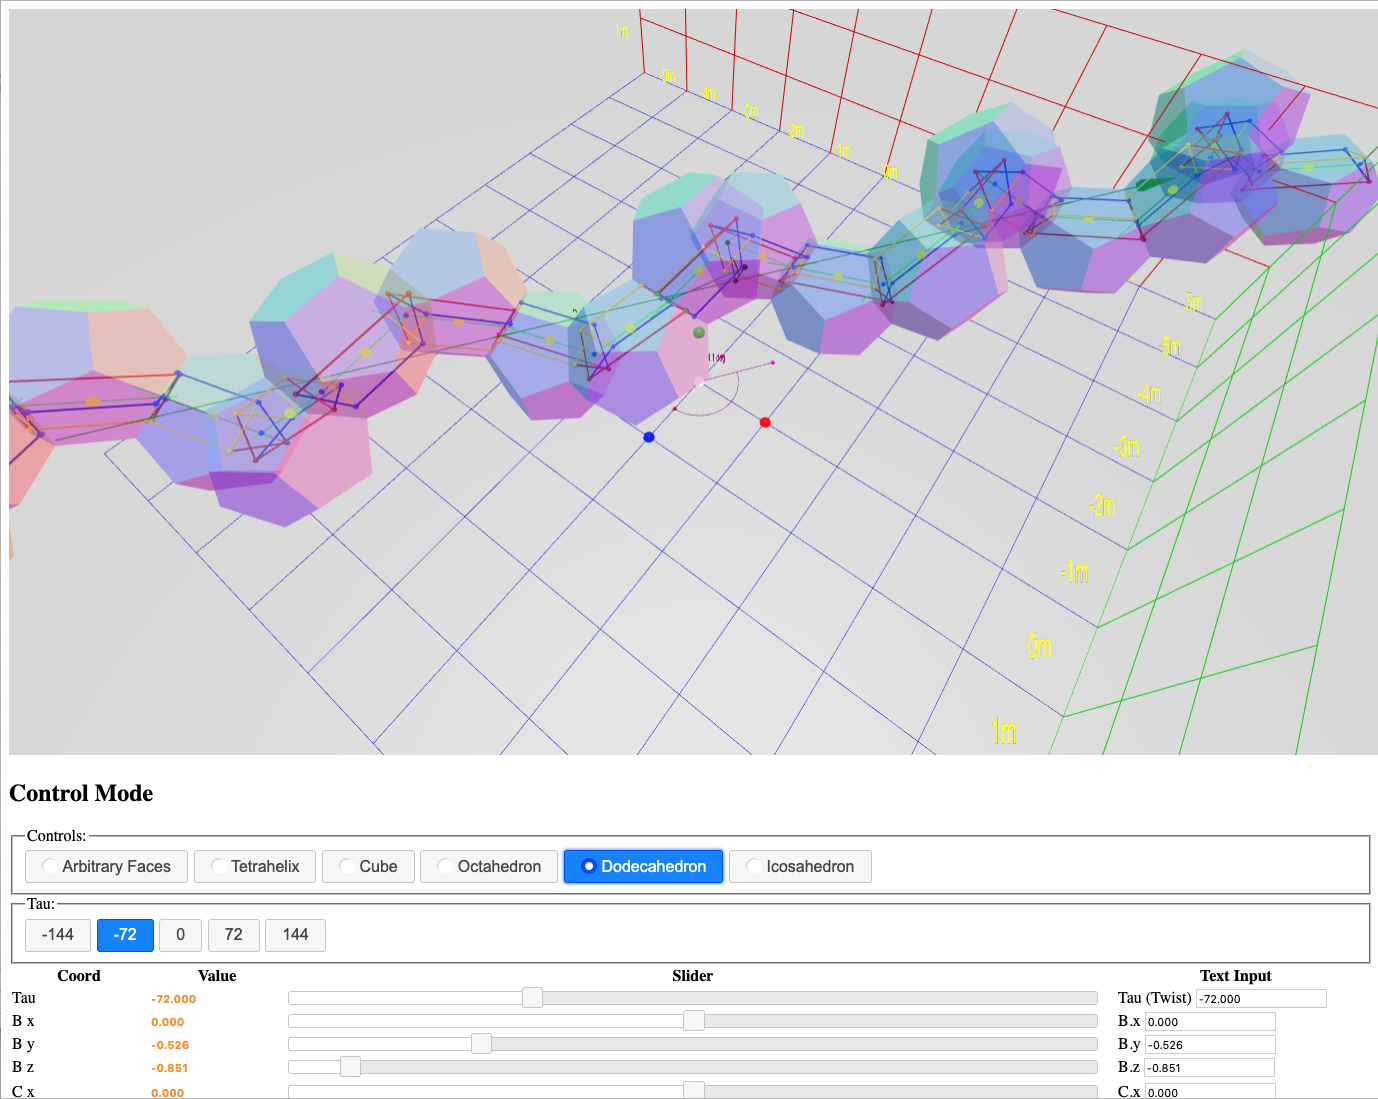
\includegraphics[width=0.80\textwidth]{figures/Dodecahedral.png}
     \caption{Example Segmented Helix Generated From the Dodecahedron}
  \label{fig:dodecahedron}
\end{figure}


\section{A Warm-up: Two Dimensions}

Considering the problem in two dimensions may be a valuable introduction.
Suppose that we consider a polygon that that as two edges, called $A$ and $B$, and that we define the length $L$ of the
polygon as the distance between the midpoints of these edges. Suppose that we are only allowed to join these
polygons by aligning $A$ of one polygon to $B$ of another polygon, with their midpoints coincident. Let us
further assume that we disallow inversions of the polygon.  Let us imagine that we have a
countable number of polygons $P_i$ indexed from $0$. Then what shapes can we make by chaining these
polygons together?

Each joint $J_i$ between polygons $P_i$ and $P_{i+1}$ will place the axes of at the same angle, $\theta$, since
our polygons do not change shape. Let us define $\theta$ to be positive
if we move anti-clockwise from $P_i$ to $P_{i+1}$ and negative if we move clockwise.
If $\theta = 0$, the joints will be collinear.

\begin{figure}
     \centering
     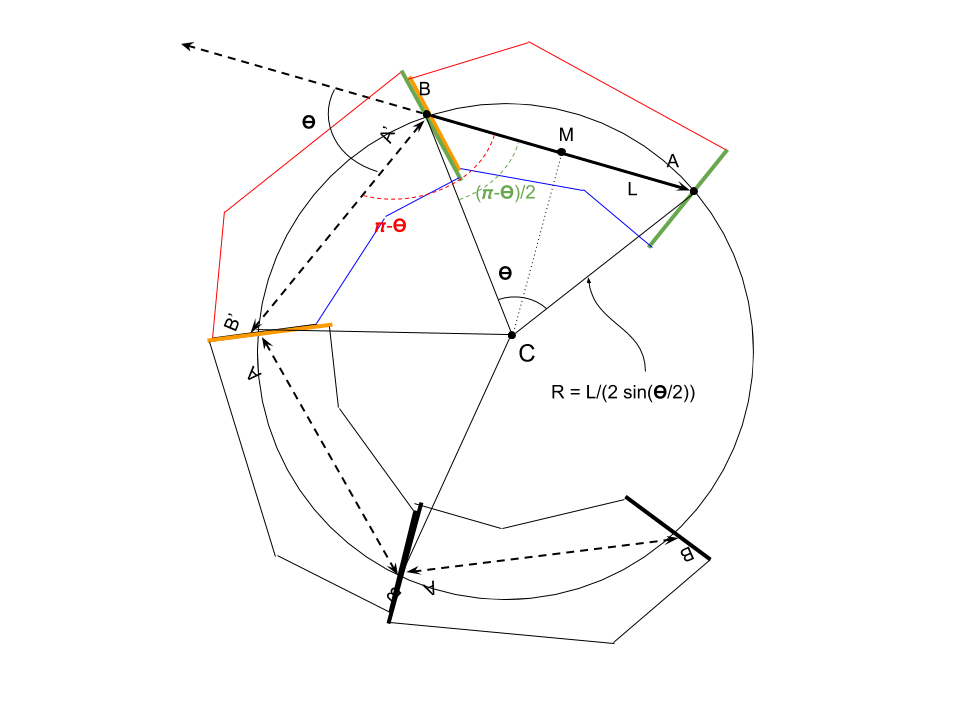
\includegraphics[width=0.80\textwidth]{figures/2DPolygonStacking.png}
     \caption{A 2D Analog of a Helix Generated by Repeated Subunits}
  \label{fig:prismdiagram}
\end{figure}

If $\theta \neq 0$, it seems they polygon joints will always lie on a circle. A proof of this
is that each polygon has associated with it an isosceles triangle $A,B,C$, where $\angle CBA = \angle CAB = \theta/2$,
and $\angle ACB = (\pi - \theta)$. $AC$ and $BC$ are not necessarily aligned with an edge of the polygon.
The length $AB$ is $L$, and the lengths $AC$ and $BC$ are
$(L/2) / \sin{(\pi - \theta)/2}$. In any chain of polygons, these triangles all meet at point $C$, and there all
joints are on the circle centered at $C$ with radius $\frac{L}{2 \sin{\frac{\theta}{2}}}$.


\label{sec:2d}

\section{The Segmented Helix}

An analogous result holds in three dimensions.

In this section we consider a helix evaluated only at regular points.

Following the Wikipedia article \url{https://en.wikipedia.org/wiki/Helix}, we set up a helix parametrically.
\begin{align*}
    P_x(t) &= r \sin{t}  \\
    P_y(t) &= r \cos{t} \\
   P_z(t) &= b t
\end{align*}
Such a helix has a radius of $r$ and slope (if $r \neq 0$) of $b/r$.
The pitch of helix, the change in $t$ needed to make one complete revolution, is $2\pi b$.
Note that a helix may be degenerate in two ways.
If $r = 0$, these equations become a line. If $b = 0$, these equations describe a circle in the $xy$-plane.
If $r = 0$ and $b = 0$, the figure is a point.

Such helices are continuous, but we are investigating stacks of discrete objects. We in fact wish to derive
the parameters for a continuous helix from such discrete objects which constrain discrete points, so we wish
to study a helix evaluated at integral points. We call such an object a {\em segmented helix}.
A segmented helix may be thought of as function that given an integer gives back a point in three space.
\begin{align*}
    P_x(n) &= r \sin{n \theta}  \\
    P_y(n) &= r \cos{n \theta} \\
   P_z(n) &= n d
\end{align*}

$d$ is the distance or {\em travel} along the axis between adjacent joints. In this canonical representation this is
the $z$-axis.
$\theta$ is the rotation around the $z$-axis
between adjacent points.
$r$ is the radius of the segmented helix.
Note that if $\theta = \pi$, we have a third form of degeneracy (to the human eye) of a segmented helix
which is a zig-zag contained completely within a single plane.

If we think of the segmented helix as describing a polyline in 3-space, we would like to investigate
the properties of that polyline. If we consider only the intrinsic shape of the segmented helix, there are three degrees
of freedom: $r,d,\theta$. We call these the {\em intrinsic} properties of the segmented helix.

\begin{figure}
     \centering
     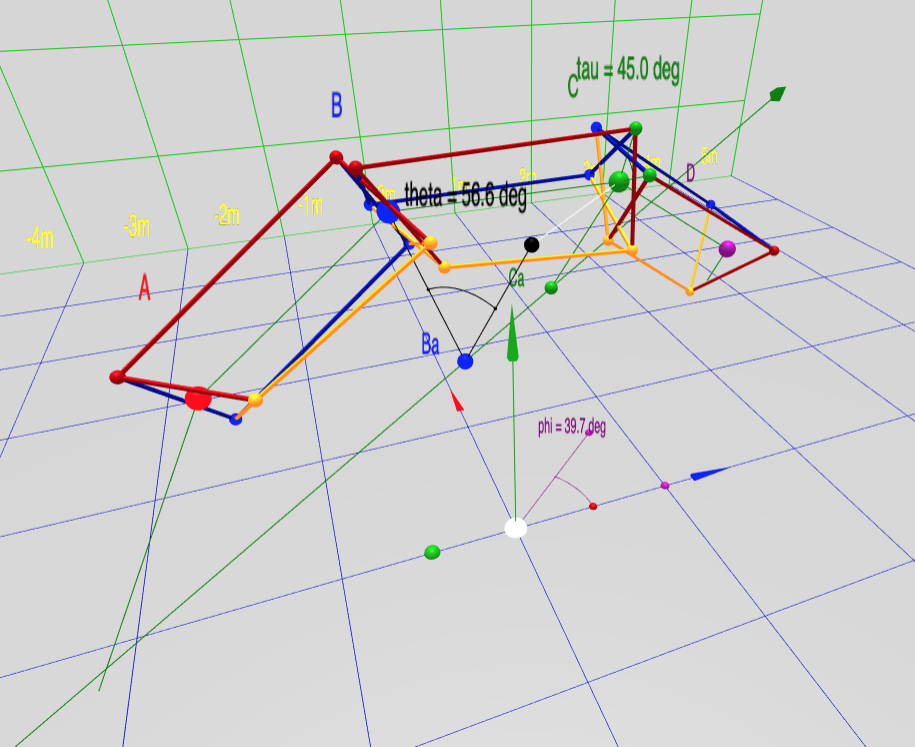
\includegraphics[width=0.80\textwidth]{figures/ABCDFigure.png}
     \caption{Naming of measures}
  \label{fig:naming}
\end{figure}

Figure \ref{fig:naming} demonstrates our conventional concepts. It is a screen shot taken from our interactive software\cite{segmentedhelixinteractive}. The
software allows parallax by supporting interactive rotation, which makes the 3D structure easier to understand; we encourage
the reader to visit our interactive page as we discuss our naming conventions.

In Figure \ref{fig:naming} and our software, we represent the object as a prism with triangular cross-section, because this is
the simplest physically realizable macroscopic object that supports a face-to-face connection. In this diagram, the
points $A,B,C,D$ are represented by the sphere of the same color as the label. The view is roughly in the direction of
the axis of the segmented helix, which is drawn as a dark green arrow, pointing in the positive $z$ and positive $x$ direction,
parallel to the $xz$ plane. For ease of viewing, the entire segmented helix has been raised by two units on the $y$ axis.
The segment $\overline{BC}$ has coordinate $y = 2$, and is aligned with the $z$-axis, and centered in $z$ direction.

The positive axes $x,y$ and $z$ axes are shown by the red, green and blue axes, respectively.
Following computer graphics convention, the $y$ axis is oriented vertically.
The points $A,B,C,D$ correspond to $P(0), P(1), P(2)$, and $ P(3)$ for a segmented helix aligned
to this axis (not the $z$-axis.)
A thin green polyvinyl represents the segmented helix, and thus connects the joints $A,B,C$, and $D$.
The points are wrapping around the axis clockwise, with an angle of $\theta = 56.6 \degree$ as
show by the on-screen protractor as the rotation from one point to the next. As will be explained in Section \ref{sec:joint}, $\tau$
is the face-on-face joint rotation of $45 \degree$.
The helix angle $\phi = 39.7 \degree$ is rendered by a protractor on the $y = 0$ plane; this the angle between the axis
and of the helix and the $z$ axis, and therefore the angle of any one segment against the helix angle.

A line is drawn from the blue point $B$ to an black sphere on the helix axis. The point on the helix axis is unlabeled
in our software, which renders it as a black sphere, but is denoted $B_a$ in this paper. Analogously, $C_a$ is the point
on the axis closest to he green point $C$.


A segmented helix located in space is completely determined by these parameters, a vector describing the axis
of the helix, and the position of any one joint.

Because the segmented helix is a discrete structure, we reframe the concept of {\em pitch} as {\em sidedness $s$}: how many segments (sides)
make a complete rotation?

The following concepts and conventional variable names for them will be related:
\begin{itemize}
\item $L$ is the distance between any two adjacent points (that is, between $B$ and $C$, for example.)
  \item $r$ is the distance between a point and the helix axis (that is, $B$ and $B_a$ for example.)
  \item $\theta$ rotation about the axis between two joints.
  \item $c$ is the length of a chord formed by the projection of the segment between two points projected along the axis of the segmented helix (A chemist may recognized this as the distance betwen residues on a {\em helical wheel} projection).
  \item $d$ is the distance along the axis of the helix between any two joints ($B_a$ and $C_a$, for example, rendered as a small black and blue
    sphere, respectively in Figure \ref{fig:naming}.
\item $\phi$ is the angle between any vector between two adjacent joints and the axis of the helix. In physical screws used in mechanical engineering, this is analogous to the {\em helix angle} \cite{wiki:helixangle}.
  \item $p$ is the pitch of the helix, the distance traveled in one complete rotation.
  \item $s$ is the number of segments in a complete rotation (in general not rational.)
\item  Finally, we find it useful to define the {\em tightness} of a segmented helix
as travel divided by radius, a number
analogous to the extension of a coil spring or slinky.
A torus-like segmented helix has zero tightness and a zig-zag has
maximum tightness. The symbol $t$ represents tightness.

  \end{itemize}
These quantities are related:
\begin{align}
    c &= 2r\sin{\frac{\theta}{2}} \\
    L^2 &= c^2+d^2  \\
    \arctan{\frac{c}{d}}  &= \phi \\
    s &= \frac{2 \pi}{\theta} \\
    d &= L \cos{\phi} \\
    p &= d s \\
    t &= d / r \\
\end{align}

Measuring $\phi$ requires us to decide on the sign of the direction of the axis, which is arbitrary and not based on the
physical shape.

Any point on on the segmented helix has a closest point on the axis of the helix. In particular, we will call the points closest to the
joints {\em joint axis points}. Then $d$ is the distance along the axis between consecutive joint axis points.

We seek to relate these properties to properties intrinsic to the joint or interface between
two segments or objects in the segmented helix. If given an object, the length between the joints $L$ is intrinsic.

\label{sec:SegmentedHelix}

\subsection{Sign Conventions for Spatially Located Segmented Helices}

When thinking about the overall shape of a segmented helix, one is
likely to be interested in the absolute magnitude of its intrinsic
properties.

However, when doing doing computer graphics work or kinematic
calculations, the sign conventions are critical. Because this
paper wishes to emphasize the continuum of shapes produced by
changing an object used to generate the segmented helix, and
in particular is interested in the degenerate helix which
produces toroidal figures, we prefer to be able to discuss
the axis of a segmented helix as a existing even when the
figure has no travel along the axis (that is, when $d = 0$).

Therefore we elect the following conventions:
\begin{itemize}
\item A right-handed coordinate system.
\item The helix as a normalized vector
  which never vanishes.
\item The travel along the axis ($d$) is negative when
  the helix is counterclockwise (that is, when motion from
  joint $n$ to joint $n+1$ appears counterclockwise when $\theta < \pi$,
  zero when toroidal, and
  positive when the helix is clockwise.
\item $\theta$ is never negative.
\end{itemize}

\section{The Intrinsic Properties of Periodic Chains of Solids}

If we have chains of repeated 3D units conjoined identically {\em periodic chains},
they generate a segmented helix coincident on their joints.
Although fairly obvious from Chasles' Theorem, we have not found this stated in writing elsewhere, so we call this Lord's Observation:

\begin{observation}[Lord's Observation]
  “In nature, helical structures arise when identical structural subunits combine sequentially, the orientational and translational relation between each unit and its predecessor remaining constant.”\cite{lord2002helical}
\end{observation}
Lord's Observation may perhaps be clarified that in fact identical objects conjoined via a rule
produce periodic chains of objects that are uniformly intersected by segmented helices and that they may be degenerate in one of
three ways that we might not strike us as a helix if we are not seeking them:
\begin{enumerate}
\item The segments may form a straight line. (For example, see Figure \ref{fig:pearlshaft}).
\item The segments may be planar about a center, forming a polygon or ring. (For example, see Figure \ref{fig:thewheel}).
\item The segments may form a planar saw-tooth or zig-zag pattern of indefinite extent (For example, see Figure \ref{fig:planarzigzag}).
\end{enumerate}

\begin{figure}
     \centering
     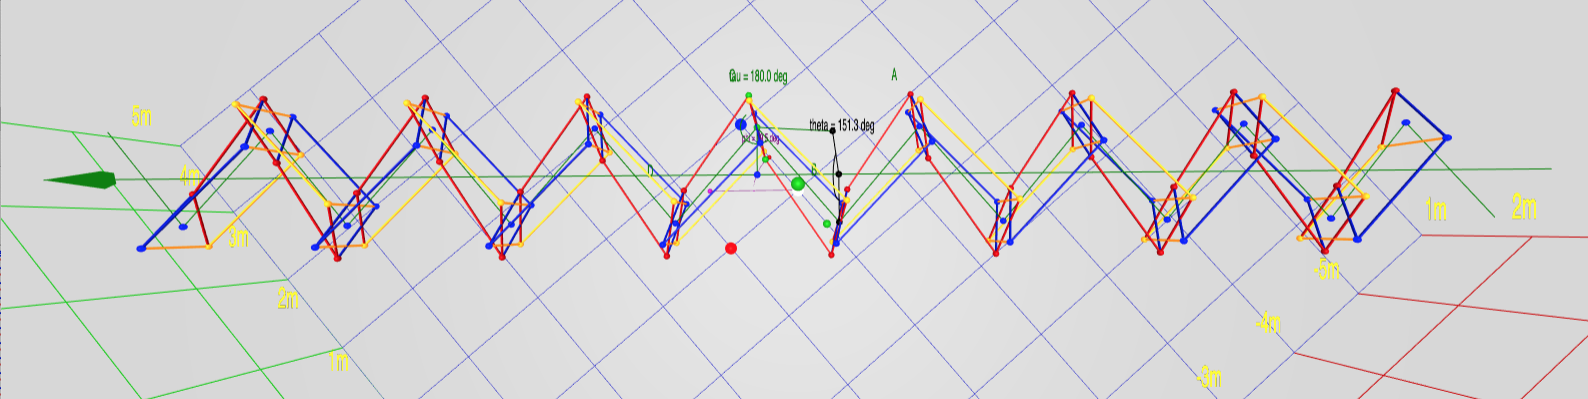
\includegraphics[width=0.80\textwidth]{figures/PlanarZigZag.png}
     \caption{A Planar Zig-Zag}
  \label{fig:planarzigzag}
\end{figure}

There are two complementary ways of learning about such segmented helices.
In one approach, we may have knowledge of the segmented helix, and
wish to learn about the subunits and the rule with which the subunits are combined.
For example, we may have microscopic objects such as proteins
or atoms, and we know from crystallography something about the positioning of these objects, without
knowing ahead of time the angles at which these objects would combine in their natural environment.
In this case, we use a variant of a linear algebra method\cite{kahn1989defining} for determining the radius, travel, and twist
of the segmented helix (these terms will be defined precisely below.)

In the other approach, we may know {\it a priori} exactly the
relevant properties of the objects and the rule which which they combine, and we seek to compactly describe the segmented helix they create.
For example, a mathematician may consider a chain of dodecahedra, or a woodworker may cut identical blocks of maple wood,
which are to be glued together face-to-face. In these cases everything about the objects and the rules for conjoining
is known before the first two objects are glued together. We call this the {\em joint face normal method}, because
it can be simulated by joining two flat faces together with a specified twist, even if the objects in question
do not actually have a physical face (such as molecules).

In both cases, we would like to understand how a change in a face normal or a twist affects the parameters
of the segmented helix,
and, conversely, we would like to be able to choose the construction of the subunits to achieve a particular segmented helix.

In engineering, sometimes the term {\em special helix}\cite{gu2012research} is use for helical curves on non-cylindrical surfaces. This paper use the term {\em helix} only in the sense of {\em cylindrical helix}.

\section{Periodic Chains Produce Segmented Helices}

A periodic chain is in fact a simple object which demonstrates tremendous symmetry.
Before using this symmetry in the construction of the segmented helix corresponding to a periodic chain, we
prove that such a segmented helix indeed exists.

\begin{theorem}[Segmented Helix]
  Consider $N$ identical objects which each have two points, $A$ and $B$, called {\em joints}. Call
  $\overrightarrow{AB}$ the {\em axis} of this object.
  Consider the frame of reference for this object to have
  its axis on the $z$-axis with $B$ in the positive direction, the
  midpoint of the at the origin, and the up-vector pointing in the positive $y$ direction.

  Consider any rule that conjoins $A$ of object $i+1$ to $B$ such that
  from the frame of reference of $i$, the object $i+1$ and anything rigidly
  attached to it is always in the same position in the frame of reference for $i$.
  Informally, $i+1$ ``looks the same'' to $i$, no matter what $i$ we choose, $i < N$.
  Call a chain of $N$ identical rigid objects conjoined via a rule that
  conjoins $A$ to $B$ in such a way that every vector
  of $B$ is always in the same position relative to a frame of reference
  constructed from $A$ a {\em periodic chain.}

  Any periodic chain of three or more objects has a unique segmented helix who
  whose segments correspond
  to the axes of these objects.
\end{theorem}

\begin{proof}
  We will proceed by induction.

  Base Case ($k == 3$):

  Take an object $AB$. By Chasles' theorem\cite{wiki:chasles}
    there is a screw axis $S$, a set of rotations,  and a transposition $d$ which moves the first object to
    position where the second object $BC$ is. Take one of the rotation angles of smallest value.
    Construct the points $A'$, $B'$ and $C'$ as the closest points
  to $A,B$ and $C$ on this axis. These points are collinear by construction.

  Now add the object $CD$ to object $BC$ by our the rule of periodic chains. Consider the points
  $B'$ and $C'$ from $A$'s frame of reference. Let $d = \| \overline C' - \overline B' \|$.
  Construct the point $D'$ on our screw axis as the point closest to $D$ on that line.

  Now because $C'D'$ in $BC$'s frame or reference must look like $B'C'$ in $A$'s frame of reference,
  the distance $\| \overline D' - \overline C' \| = d$.
  From $A$'s frame of reference, $A'B'C'$ are collinear, the points $B'C'D'$ must be collinear in
  $B$'s frame of reference.

  In any frame of reference, if $A'B'C'$ are collinear and $B'C'D'$ are collinear, then $A'B'C'D'$
  are collinear.

  Now, looking backward from $CD$ towards $A$, the distance $A'B'$ must be the same as the
  distance $B'C'$ so as to not violate our rule. So $d = \| A'B' \| = \| B'C' \| = \| C'D'\|$.
  Similarly because by construction $r = \| B B' \| = \| C C' \|$, and $AA'$ is a rigid
  transformation of $BB'$, so $r = \| A A' \|$. By symmetry, $r = \| D D' \|$.
  Compute $\theta$ as the rotation about $S$ that takes $B B'$ into $C C'$. By our rule
  of attachment, $\theta$ also takes $C C'$ into $D D'$ and $A A'$ into $B B'$.

  Now construct a segmented helix, the radius $r$, distance,
  and angle $\theta$. This segmented helix can be positioned coincident with $S$ so
  that $H_0 = A$. Then $H_1=B$, $H_2=C$, and $H_3=D$.

  Therefore, for the base case of three objects, there is a segmented helix whose
  segments coincide with the axes of the objects.


  Inductive Case ($k+1$):
  Assume there is a segmented helix coinciding with the first $k$ objects, and
  consider the frame of reference of the $k$th object. The axis and any
  other rigid property of the $k+1$th object stands in relation to object $k$
  as $k$ stood to $k-1$. By induction, the $k$th object had a segment
  of a segmented helix corresponding to its axis. Attach vectors $V_{Ak}$ and $V_{Bk}$
  from the
  joints of $k$ to the axis of the helix perpendicularly. Define these
  vectors in the frame of reference for $k$.

  To the $k-1$th, the tips of  $V_{Ak}$ and $V_{Bk}$ define
  a line segment which lies on the axis of the segmented helix $H$, with the
  tip of $V_{Ak}$ coincident with the tip of $V_{B(k-1)}$.

  By our rule and by induction, since this is true of the $k-1$th object,
  it is true of the $k$th object. Therefore the $k+1$th objects $V$ vectors
  point to a line segment which lies on the axis of $H$, extending it
  in the same direction. The axis of the $k+1$th object therefore coincides
  with the $k+1$th segment of $H$.

  Therefore, by induction, identical objects conjoined by the same rule always
  coincide with some segmented helix, whose parameters are discoverable.
\end{proof}

This theorem leads to the following corollary. In engineering the term {\em helix angle} refers
to the angle between a line tangent to a continuous helix and
the axis of the helix. In segmented helices, this is the same
as the angle between the
axis of each object in a periodic chain and the axis of the
  segmented helix coincident to it.
\begin{corollary}[Segment Similarity]
  The helix angle of a any object axis in a periodic chain is the same.
  \label{cor:symmetric}
\end{corollary}

\begin{proof}
  The axes of each object coincide with a segment of a segmented helix.
  A segmented helix is completely symmetric no matter in which direction
  of the axis you look down or which point on the axis you begin at. The angle between each pair of objects
  is exactly the same.
\end{proof}

Corollary \ref{cor:symmetric} is perhaps not obvious when one considers
period chains of objects which are, taken as individuals, highly asymmetric.
For example,
The $B$ face does not have to be the same size as the $A$ face. In fact,
the object itself might be shaped like the letter ``C'', and not completely
enclose the axis. Taking the idea further, the object might be spiky
like a stellated polyhedron or a sea urchin, and still be joined by
joints relatively close to the center of the object. In this paper
we do not concern ourself with the issue of self-collision of the objects,
which would have to be considered if one attempted to make a period chain
of sea urchins.

Corollary \ref{cor:symmetric} will be used in our development of {\em PointAxis} algorithm
and in our computation of segmented helix properties and to justify balancing face normals
to produce an intrinsic out-vector and to apply the {\em PointAxis} algorithm
without actually assigning objects Cartesian coordinates.

\section{Computing Screws and Segmented Helices from Transformation Matrices}

The rule for how objects in a periodic chain are joined may be conveniently captured as a transformation
matrix. In general, a human engineer will have to compute this transformation matrix from some other
information, such as the face-to-face conjoining rule. We discuss how to do this from joint-face normal
vectors in Section \ref{sec:facenormal}. However, a transformation matrix clearly
capture the idea of ``repetition''. Since by definition the objects in the chain are the same shape,
moving one object into a new position and place an identical copy of that object in that position
are practically the same.

Using standard screw theory\cite{wittenburg2016kinematics,wiki:screwaxis}, a screw can be computed from such
a transformation matrix. This consists of the axis of the screw $S$, a point on the screw axis $P$,
the rotation $\theta$ around the axis, and the
transposition, or travel, along the axis of one transformation.

Neither a transformation matrix or its corresponding screw
completely define all of the intrinsic
properties of a segmented helix. In particular, a matrix $M$ maps any point $p$ to a point $p'$.
Since this applies to all points no matter how far from the screw axis or the axis of rotation and
such transformation preserve distance to this axis (the radius), the radius is of a segmented helix
is not determined by a transformation matrix or a screw. Since the helix angle $\phi$ changes
with radius for a helix of a given pitch, $\phi$ is not determined.

However, if we have a screw and one point on the axis of the screw fixing it in space
and the location of one joint, all of the properties of the segmented helix are completely determined.

In our software, we have coded the calculation of the screw directly from a transformation matrix, and
the additional routines which determine all intrinsic properties from a joint position (making
certain arbitrary alignment choices without loss of generality.)

Although not original to this paper, the author found it
difficult to find clear documentation on how to calculate the
screw from the transformation matrix.
We therefore include an exposition here, in hope it will be useful,
and a valuable adjunct to the code to a programmer seeking to duplicate
this functionality.

\subsection{Computing the Screw Axis from a Transformation Matrix}

Our goal is to compute a normalized vector $\hat{u}$ aligned with the screw
axis of the transformation effected by a transformation matrix $R$.

In order to be robust, it is valuable to check that the transformation
matrix is a rigid transformation\cite{wiki:rigid},
as Chasles' theorem applies only to rigid transformations.

The angle of rotation is computable from the trace of $R$, $Tr(R)$.
\begin{align}
  \theta &= \arccos{\frac{Tr(R) - 1}{2}}
\end{align}
Technically, $\arccos$ is multi-valued, but we will take $\theta$
to be in its principle range, $0 \leq \theta leq \pi$.
If $\theta$ is $0$ or a multiple of $\pi$, then we the {\em zig-zag}
degenerate case, the method of compute $H$ from the rotation
basis of $R$ is numerically unstable. However, in this case
we can compute the direction vector $H$ as the difference vector
between an arbitrary point $P$ and its transformation performed
twice. Informally, this is a ``zig, then a zag''.
\begin{align}
  H &= (R ( R( P))) - P
\end{align}
(Note that in general $H$ is not normalized, $H \neq \hat{H}$.
Also recall that multiplication by a transformation matrix
produces a point that in a new position representing
the transformation.)

In other cases, $u$ can be computed from the direction
cosines of $R$\cite{wiki:rotation}:
\begin{align}
  R &=     \begin{bmatrix} a & b & c' & x \\ d' & e & f & y\\ g & h & i & z\\ 0 &  0 & 0 & 1\end{bmatrix} \\
    H &=  \begin{bmatrix} h - f \\ c' - g \\ d' - b  \end{bmatrix}
\end{align}
(The variables $c'$ and $d'$ are marked to distinguish them from
the symbols for the chord $c$ and the travel along the axis $d$.)
The magnitude of $\norm{H} = 2 \sin{\theta}$, which vanishes
when $\theta$ is $0$ or multiple of $\pi$, hence our need
to treat those cases differently.

Although the matrix $R$ in general produces both a rotation
and a translation in space, distance between $P$ and $R(P)$
in general depends on how far $P$ is from the axis of rotation.
However, the travel $d$ along the axis of the rotation does
not depend on $P$. It can be computed as a dot product:
\begin{align}
  d = \overrightarrow{BC} \cdot \hat{H}
\end{align}

These are the only properties that can be computed from the
matrix $R$ alone; but once we have the length along the
object axis ({\em not} the helix axis) $L$ of an object
we can compute our computations, based on relations
already given in Section\ref{sec:SegmentedHelix}.

The chord of the segmented helix (that is, length of an object of
axis length $L$
projected along $H$) is:
\begin{align}
  c = \sqrt{L^2 - d^2}
\end{align}
Knowing the chord $c$ and the amount of rotation $\theta$
allows us to compute the radius:
\begin{align}
  r = \frac{c}{2 \sin{\theta}}
\end{align},
unless the chord is $0$, in which case the radius is $0$.
The helix angle $\phi$ is a a function of $c$ and $d$:
\begin{align}
    \phi &= \arctan{\frac{c}{d}}
\end{align}

Sidedness and pitch ($s$ and $p$) follow directly.

Finally, the vector $\hat{H}$ gives the direction of the
axis of the helix, but does not give us a point which fixes
it in space. It is most convenient to accept a point $B$
which is a joint and produce the point $B_a$ which is the
point on the helix axis closest to $B$.

To do this, we conceptually construct the midpoint $M$
of $\overrightarrow{BC}$ and utilize the fact that the vector $Q$
from it to its closest point on the axis $M_a$ is perpendicular
to the containing both $\overrightarrow{BC}$ and $H$. Therefore
its direction is constructible via cross product, and
its length $l$ is computable from the radius and chord. $M_a$
is the midpoint of $B_a$ and $C_a$, so we can just move back
half the travel $d$ along the vector $u$ to get $B_a$.

\begin{align}
  C &= R(B) \\
  \overrightarrow{BC} &= C - B\\
  M &= \frac{B + C}{2} \\
  Q &= \overrightarrow{BC} \times u \\
  l &= \sqrt{r^2 - \frac{c}{2}^2} \\
  Q' &= -\frac{Q}{l} \\
  B_a &= M + Q' - \frac{d}{2}\hat{H}
\end{align}

Thus given only the transformation $R$, the length $L$, and one
joint $B$, one may compute all of the intrinsic properties
($r,\theta,d,c,\phi$) of
the segmented helix and positioned it in space via $H$ and $B_a$.

As is common in kinematics\cite{funda1990computational}, there are many ways to represent
the same physical or mathematical situation.
Four consecutive joint positions also completely determine a segmented helix, as presented below.
Because joints can be computed from transformation
matrices and transformation matrices from joints,
which method of calculation is preferable would be
a matter of choice and clarity. We have
in fact coded both and used the comparison as automated tests in
our software to ensure
the correctness of our coding.

A mechanical engineer, robotocist, or computer graphics expert is
likely to find the computation from the
transformation matrix more natural and convenient.
A chemist or crystallographer is more likely to
have learned the position of four points and wish to compute from that.

\section{{\em PointAxis}: Computing Segmented Helices from Joints}

\begin{figure}
     \centering
     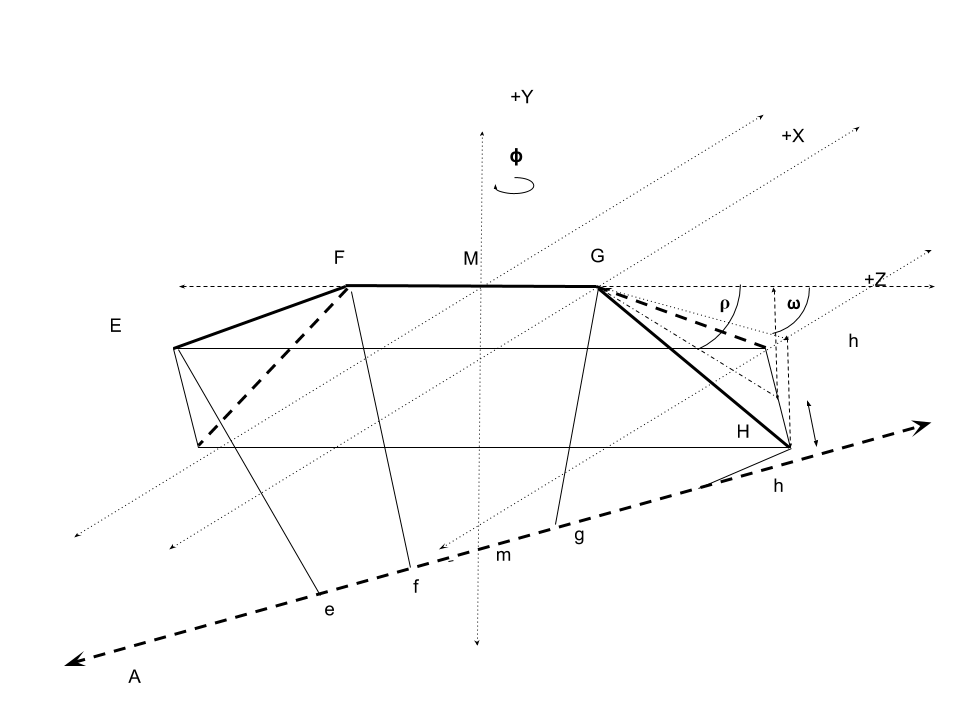
\includegraphics[width=0.80\textwidth]{figures/TwoAngleDiagram.png}
     \caption{Three Symmetric Members}
  \label{fig:threemembersdiagram}
\end{figure}

Kahn\cite{kahn1989defining} has given a method for computing
the axis of a helix in the context of chemistry.
This method uses the observation that the angle bisectors
of the segments on a segmented helix are perpendicular
and intersect the axis of the helix.
Because the helices may not be perfect and because the measurement of positions may not be perfectly accurate,
it is common for chemists to use regression and fitting methods to fit helix parameters to observed positions
on the helix.
Kahn's method was a prelude to some error-tolerant methods applicable to
the realm of organic chemistry.
In this paper we are concerned with pure geometry. Also, Kahn was writing in 1989,
and we now have more convenient computing tools. We give here a modification of Kahn's algorithm, called {\em PointAxis},
which relies on our ability, working in the realm of pure geometry, to position the segments on the axes
to simplify the derivation and computation.

\subsection{A Sketch of the 4-Point Method}

Using tools from linear algebra and well-documented algorithms, a sketch of the finding the segmented helix from
four consecutive known points $A,B,C,D$ is:
\begin{itemize}
\item Compute the bisectors of the angle $B_b$ of $ \angle{ABC}$ and the angle $C_b$ of $\angle{BCD}$.
  If the points are collinear, we have a special case.
\item Because these angle bisectors point at the axis of the segmented helix, their cross product is a vector
  in the direction of the axis. If $B_b$ and $C_b$ are parallel or anti-parallel the cross product is not defined
  and we have special cases.
\item  Otherwise the vectors $B_b$ and $C_b$ are skew, the algorithm for the closest points on
  two skew lines provides two points $B_a$ and $C_a$ on these vectors which
  are the closest points on on those lines and are also points on the axis.
\item The distance between $B_a$ and $B$ is the radius, and the distance between $B_a$ and $C_a$ is the travel $d$ along the axis.
  \item The angle between $\overrightarrow{B - B_a}$ and $\overrightarrow{C - C_a}$ is $\theta$.
  \end{itemize}


\subsection{The 4-Point Method}

Therefore four consecutive points completely determine at least one segmented helix. We will concern ourselves
only with the helix that makes the least rotation between points.
We provide a modification of the {\em PointAxis} algorithm
with takes four such points (without loss of generality $B$ and $c$ are assumed to be centered on the $z$-axis, and that a
rotation has been performed to balance $A$ and $D$ to that $A_x = -D_x, A_z = -D_z$, and $A_y = D_y$. Thus the input to
{\em PointAxis} in fact has three only three degrees of freedom, which determine the three intrinsic properties $r,d,\theta$
which completely define the shape of a segments helix (but not its location in space.) A practitioner may be able to set up
the coordinate system such that the four points are in balance;
if not, Section \ref{sec:balance} discuss how to transform them
into balance.

\begin{figure}
     \centering
     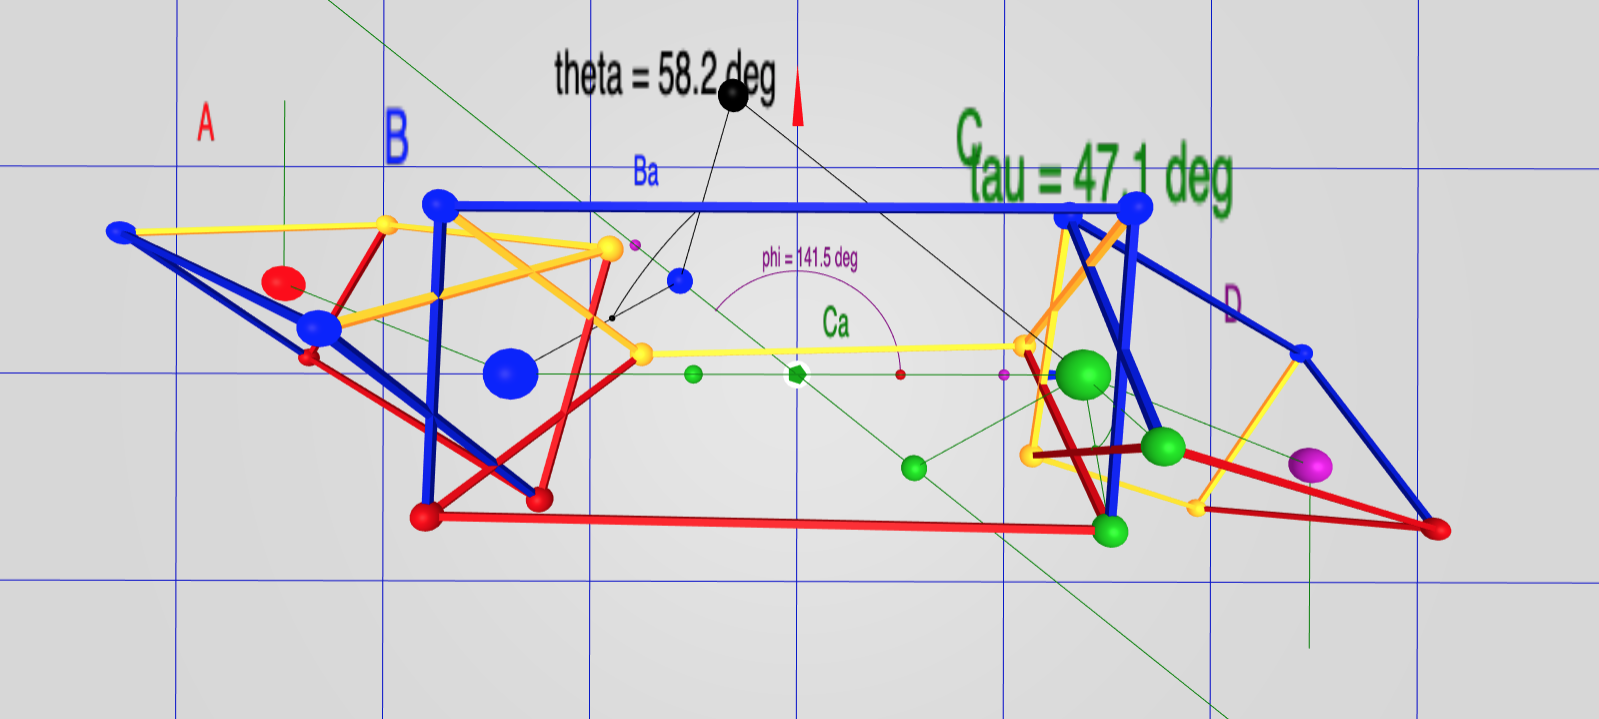
\includegraphics[width=0.80\textwidth]{figures/Balance.png}
     \caption{A Balanced Configuration}
  \label{fig:balancediagram}
\end{figure}

Figure \ref{fig:balancediagram} shows a downward view of a balanced configuration (though raised above the origin
instead of at the origin.) $A$ (the red sphere) is a reflection of $D$ (the purple sphere) across
the midpoint. Both $A$ and $D$ are hanging downward. If the structure where hung on a point at the origin, it would
be physically balanced. Note it is always possible to achieve this balance, even thought the object
itself is not symmetric; in this figure the normal of the $B$ face is not symmetric with $C$ face.


In the derivations below, we rely on certain facts about
the segmented helix formed by the stack of objects, the first
of which is key:
\begin{itemize}
\item Without loss of generality, we may think of any member whose faces
  and twist generate a non-degenerate helix as being ``above'' the
  axis of the helix. We furthermore choose to place the object in
  this figure so that $B_y = C_y$, that is, that the members are symmetric
  about the $z$-axis.
  $A$ and $D$ are ``balanced across the $YZ$-plane,
  and $A_x = -D_x$ and $A_y = D_y$.
\item Every joint ($A,B,C,D$) is the same distance $r$ from the axis $H$ of the helix.
\item Every member is in the same angular relation $\phi$ to the axis of the helix.
\item Since every member cuts across a cylinder around the axis,
  the midpoint of every member is the same distance from the axis
  which is general a little a less than $r$. In particular the midpoint $M$
  whose closest point on the helix axis $m$ is on the $y$-axis and
  $\overline{Mm} < \overline{Bb}$.
\item The points ($A_a,B_a,C_a,D_a$) on the axis closest to the joints ($A,B,C,D$)
  are equidistant about the axis and centered about the $y$-axis. In
  particular, $\| \overline{B - B_a} \| = \| \overrightarrow{C - C_a} \|$.
\end{itemize}

From the observations that $\| \overrightarrow{B - B_a} \| = \| \overrightarrow{C - C_a} \|$
we concluded that the helix axis is in a plane
parallel to the $XZ$-plane, it intersects the $y$-axis, but in general is
not parallel to the $z$-axis.

Because the angle bisectors of each joint are in general skew, and intersect the
axis perpendicularly, it is clear we can use linear algebra and the algorithm
for the closest points on two skew lines to find $B_a$ and $B_c$.

However, we can take advantage of the fact that a segmented helix has
tremendous symmetry, and the angle bisectors are very far from being two
generally skew lines. In fact, by taking advantage of the fact that the
generating rule for an object chain requires similarity in every joint,
we can arrange the objects as in Figure \ref{fig:threemembersdiagram}.

{\em PointAxis} takes a length and a point $D$ known to be in
a specific relation to $B$ and $C$.

We have carefully arranging our axes
so that we can compute $\phi$, the angle between the helical axis
and the $z$ axis. This, in combination with symmetry and the knowledge
that the helical axis is in the $XZ$ plane, lets us compute the
points on the axis corresponding to the joints directly from $\phi$.

This algorithm coded below is simple enough that Mathematica\cite{Mathematica} can
actually produce symbolic closed-form formula for all computed valued
in terms of $L, x, y, z$, but they are less comprehensible to the
human eye than this algorithm, although their existence opens
the possibility that, for example, the derivative representing
the change in $r$ with a change in $D$ could be calculated.

\subsection{Degenerate Cases}

Define the angle bisector vectors:
\begin{align}
  B_b &= B - (A + C)/2 \\
  C_b &= C - (B + D)/2 \\
  \end{align}
The fundamental insight that the axis of the helix $H$ can be
computed by a cross product of the angle bisector
vectors ($B_b$ and $C_c$) applies only
when the angle-bisectors have a non-zero length and when
they are not anti-parallel. When the are of zero length, this is
the degenerate case of a straight line coinciding with all segments.
In this case the segmented helix has
This occurs only when $A_x = 0 \wedge A_y = 0 \wedge A_z = -3L/2$.
In this case:
\begin{align}
  r &= 0 \\
  \theta &= \text{undefined}\\
  d &= L \\
  c &= 0 \\
  \phi &= 0 \\
  H &=  \begin{bmatrix} 0 \\ 0 \\ L  \end{bmatrix} \\
  B_a &= B = \begin{bmatrix} 0 \\ 0 \\ -L/2  \end{bmatrix}
\end{align}
$H$ is the direction vector of the helix axis.
In this case we do not have enough information to define $\theta$,
unless it is through other information. For example, when using
the joint-face normal method which specifies
the twist $\tau$ at the faces, then $\theta = \tau$.

When $B_b$ and $C_b$ are parallel (pointing in opposite directions),
the zig-zag degeneracy occurs. Since we are assuming
the balance of $A$ and $D$, this occurs only when $A_y = 0$.
In this case (denoting the $x$ component of the $B_a$ vector as $B_{a[x]}$):
\begin{align}
  B_{a} &= \begin{bmatrix} B_{a[x]} \\ B_{a[y]} \\ B_{a[z]}  \end{bmatrix} \\
  H &=  C - A \\
  d &= (C - B) \times H \\
  r &= \norm{B_b} / 2 \\
  c &= 2 r\\
  \phi &= \atantwo{(H_z,H_x)} - \pi/2 \\
  c &= 0 \\
  \theta &= \pi \\
  B_{a[x]} &= \frac{d\sqrt{1 - (d/L)^2}}{2} \\
  B_{a[y]} &= 0 \\
  B_{a[z]} &= -\frac{d^2}{2L} \\
\end{align}

However, the most general case is simpler, and can be worked
out with standard linear algebra operations. In the math below
which is a direct analog of our coded solution, we have
utilized the tremendous symmetry of the ``balance'' condition
to use mostly scalar operations. There is some hope that
this would allow closed-form expressions to be produced, perhaps
with the aid of a symbolic computation system such as
Mathematica\cite{Mathematica}. If completed, this would
allow us to give closed-form solution to the intrinsic properties
of all the 28 Platonic helices enumerated in Sec\ref{sec:platonic}.

Once $H$ has been calculated, the signed travel along the axis $da$ is
the scalar projection of a segment $(C - B)$ onto $H$.
From this $\phi$ is directly calculatable. $\phi$ allows
a direct calculation of the $x,y$ and $z$ components of the
point $B_a$ on the axis pointed to by $B_b$.
$r$ is the distance between $Ba$ and $B$. $c$ and $\theta$
are easily computed from these values.

\begin{align}
  H &=  \begin{bmatrix} -2 B_{b[y]} B_{b[z]} \\ 0 \\ 2 B_{b[y]} B_{b[x]}  \end{bmatrix} \\
  d &= \frac{L B_{b[x]}}{\sqrt{B_{b[x]}^2 + B_{b[z]}^2}}  \\
  \phi &= \atantwo{(H_z,H_x)} - \pi/2  \\
  c &= \sqrt{L^2 - d^2} \\
\end{align}

In this approach to calculation, it is easiest for
us to compute the axis point $B_a$ corresponding to $B$ and
use it to complete our computations.

From trigonometry and utilizing the facts that $\phi = \arccos{d/L}$
and that $\sin{\arccos{x}} = \sqrt{1 - x^2}$ it
can be shown that
the $x$ and $z$ component of $B_a$ are:
\begin{align}
  B_{a[x]} &= \frac{d\sqrt{1 - (d/L)^2}}{2} \\
  B_{a[z]} &= -\frac{d^2}{2L}
\end{align}

However, this computation exposes another special case: when the
helix angle $\phi$ is $\pi /2$, the segmented helix is
a torus-like. In this case the axis point $B_a$ is in fact
on the $y$-axis, and we need only compute $B_{a[y]}$:
\begin{align}
  B_{a[y]} &=  \frac{L B_{b[y]}}{2 B_{b[z]}}
\end{align}
When we are not toroidal, we must take $B_{b[x]}$ into
account, but it is non-zero, so we can divide by it.
By imagining a plane pressed downward from the
object axis to the helix axis, we see that $B_{a[y]}$
is proportional to a ration of the angle bisector
$B_{b[y]}/B_{b[x]}$ times the $B_{a[x]}$ value:
\begin{align}
  B_{a[y]} &=  \frac{ B_{b[y]} B_{a[x]}}{ B_{b[x]}}
\end{align}

Having computed all of $B_a$, the remaining intrinsic properties are easily
calculated:

\begin{align}
  r &= \norm{B - B_a}  \\
  \theta &= 2 \arcsin{\frac{c}{2r}} \\
\end{align}


\subsection{The 4-Point Test}

It is useful to have a test if four proposed points really do lie on a segmented helix, to see
if they allow valid inputs to {\em PointAxis} algorithm to be computed via rigid transformation to the $z$-axis.

\begin{theorem}[Segmented Helix Test]
  Four arbitrary sequential points $A,B,C,D$ are consecutive joints of a segmented helix if and only if
  they segments $\overline{AB},\overline{BC}$, and $\overline{CD}$ are equal length and the scalar projection
  of $\overrightarrow{CD}$ onto $\overrightarrow{BC}$ is equal to the negation of the scalar projection of $\overrightarrow{AB}$
  onto $\overrightarrow{BC}$.
\end{theorem}

\begin{proof}
  ``If'' Case (points on helix imply scalar projections are negations of each other):
  If $A,B,C,D$ are consecutive joints on a segmented helix, then the angle $\eta$ between any two consecutive segments is the
  same. Then:
  \begin{alignat*}{2}
    \norm{\overrightarrow{AB}} &= \norm{\overrightarrow{CD}} &\quad &\text{Given}\\
    \norm{\overrightarrow{AB}}\cos{\eta} &= \norm{\overrightarrow{CD}}\cos{\eta} &\quad &\text{$\eta$ the same for each joint} \\
    \overrightarrow{AB} \cdot \hat{\overrightarrow{BC}} &= \overrightarrow{CD} \cdot \hat{\overrightarrow{BC}} &\quad &\text{def. of scalar product} \\
  \end{alignat*}

  ``only if'' Case (equal scalar projections and length imply coincident segmented helix):

  If the scalar products and the lengths are equal, then the cosines of the angles between segments are equal. In the range $0$ to $\pi$,
  $\cos{\theta} = \cos{\phi}$ implies $\theta = \phi$. Therefore the angles between the segments are equal.

  By the previous argument of correctness for the {\em PointAxis} algorithm, a rigid transformation always exists
  which balances three such segments, there always exists a helix axis that
  is in the $xz$ plane the intersects the $y$ axis and is the same distance from $A$, $B$, $C$ and $D$.
  This axis is the axis of a segmented helix which rotates each point similarly, provides the same translation along the axis,
  and maintains the same radius. Hence a segmented helix exists whose joints are $A$, $B$, $C$, and $D$.
\end{proof}

\subsection{Comparison}

There is one reason one might prefer the transformation matrix method or the point method over the other: with modern
computer algebra systems such as Mathematica\cite{Mathematica} it might be possible to use these ``algorithms'' to produce closed-form
expressions of closed-form (algebraic) inputs. For example, the Platonic solids all have lengths and face normals which
can be specified exactly in closed (thought irrational) form. Thus it might be possible to produce an expression for the
radius of one of the Platonic Dodecahelices of unit edge length. We have not undertaken this work.


\section{The Joint Face Normal Method}
\label{sec:facenormal}

{\em PointAxis} takes a point $A$ known to be in a specific, balanced relation
to $B$ and $C$. A chemist might know 4 such points from crystallography,
and be able to move them into this symmetric position along the $z$-axis.

However, we might instead know something of the subunits and
how they are conjoined, without actually knowing where points $A$
and $D$ are.

We start with these intrinsic properties of an object, and additionally the
rule for how objects are laid face-to-face. That is, knowing the length between two
joint points and a vector normal to the faces of the two joints, we almost have
enough to determine the unique stacking of objects. The final piece is that we must
know the {\em twist}. That is, when face $A$ of a second objects is placed on face $B$
of a first object so that they are flush (that is, their normals are in opposite directions),
it remains the case that the second object can be rotated about the normals. To
define the joining rule, we must attach an {\em up vector} to each object. Then a joining
rule is ``place the second object against the first, joint point coincident to joint point,
and twist it so that its up vector differs by $\tau$ degrees from the up vector of the first
object.'' In this definition, the up vectors are considered to be measured against the plane
containing the two axes meeting in a joint.

Define the {\em joint plane} to be the plane which contains the two axes meeting in a joint.
Define the {\em joint line} to be the line through the joint perpendicular to the joint plane.
Define the {\em joint angle} to be the angle of the first axis to the second measured about
the joint line.
The twist $\tau$ is the change in the a vector attached to the object rotated about the joint
line by the joint angle. That is, take any vector attached to the first object, place it at
the joint, rotate it about the joint line via the joint angle. $\tau$ is the difference
between the angle of this vector measured against the joint plane and the angle of the
up vector of the second object measured against the joint plane.

If the objects are macroscopic objects which have faces, this is the same as the rotation
of the axis of the second object relative to the first in the plane of the coincident faces.
We can identify intrinsic properties:

\begin{itemize}
\item An object with two identified faces, labeled $B$ and $C$. Assume there normalized
  vectors $N_B$ and $N_C$
  from each of these points that is aligned with the axis of the conjoined object attached to
  that face. This normals might be enforced by the fact that flat faces are joined in the joint plane.
  However, molecules don't have faces; this conjoining relationship may be enforced some other way.
\item The length $L$ of an object, measured from joint point $A$ to joint point $B$.
\item A joint twist $\tau$ defining the change in computed out-vector between objects,
  measured at the joint face.
\end{itemize}

\subsection{Rotating into Balance from Face Normal Vectors}

\label{sec:balance}

In order to use the {\em PointAxis} algorithm, we need a way
to compute points $A$ and $D$ in balance around the axis $BC$.
A key insight is that Lord's Observation tells us that no matter how lopsided and different
the normal vectors  $N_B$ and $N_C$ for the joint faces are and no matter what $\tau$ we choose,
when we conjoin objects
their relationship is always the same.
After placing $BC$ along
the $z$-axis, there is always an angle $\psi$ which will
rotate the points $A$ and $D$ into balance (that is, $(A_x = -D_x) \wedge (A_z = -D_z) \wedge (A_y = D_y)$.

For computer programmers with a graphics library supporting transformation matrices such
as THREE.js\cite{dirksen2013learning},
it is relatively easy to code the math to adjoin objects
face-to-face based on the face normals, simulating the physical act of
matching flat faces between macroscopic objects.
\begin{enumerate}
  \item Create the transformation the aligns and centers $\overrightarrow{BC}$ on the $z$-axis.
\item Create a translation of $B$ to $C$.
\item Create a rotation of the $z$-axis to  $N_B$.
\item Create a rotation of of $-N_c$ about $N_B$.
  \item Create a rotation of $\tau$ around that axis.
\end{enumerate}
Composing these transformation matrices via multiplication creates a
transformation matrix which takes $B$ to $C$ and $C$ to $D$.

We will assume this
as a subroutine called {\em adjoinPrism} which takes $\tau$
(the rotation inside the plane of the joint). A byproduct
of balancing the points is the a transformation matrix
that takes $C$ into $D$. Having done this, one can compute
the screw axis, and hence all of the segmented helix properties,
from either the transformation matrix or the four points. Our
code does both and compares the result as a test.

\subsection{The Key to Balance}

The key insight to finding $\psi$ to note that we
can consider the projections of the $B$ and $C$ face normal vectors
projected into the $XY$ plane, and rotate these so that they
are balanced around the negative $y$ unit vector.
Such a projection into the cross-section of the helix is closely related to
the {\em helical wheel}\cite{wiki:helicalwheel} plot
in the study of alpha helices in proteins.
Even if the lengths of the projections of the face normals in $XY$
are different, this mechanism works, because by Lord's Observation
the points $A$ and $D$ must be symmetric about the segment $\overline{BC}$.

By composing this balancing operation with the face-adjoining transformation
matrix, $A$ and $D$ are placed in balance. The screw axis may now
be computed from either the four points $A,B,C,D$ or from the transformation
matrix created to balance them.

\subsection{On the Choice of the Screw Axis Direction}

Given only a physical segmented helix without position in space, we may arbitrarily choose the
direction for the axis. Changing our decision will make the screw axis point in the negative direction,
change the sign of the travel $d$ along the axis, and choose $\phi$ to be $\pi - \phi$.

As can be seen from interactive play with our software\cite{segmentedhelixinteractive}, it is entirely possible for the travel along
the axis of the helix to be $0$--in fact, choosing $\tau \approx 0$ produces toruses, which have no
travel along the axis.

We could represent this be making the length of the vector representing the axis be the length of the
travel $d$. However, this would have the drawback than when $d$ is zero we would be unable to determine
the axis of revolution of the torus. Although somewhat arbitrary, we have chosen instead to represent the
axis as a normalized vector of unit length, and to allow the travel to be negative. This has the benefit that
changing $\tau$ through (something close to) zero smoothly changes $d$. However, it creates the problem that as $\tau$ approaches
(something close to) $\pi$ from different directions the signs of the axes are different.
That is, $\tau \approx \pi$ and $\tau \approx -\pi$ describe exactly
the same shape, but in our calculation they will have different signs for the axes. The radius, pitch and
absolute value of the travel,
which are intrinsic to the shape, will be the same, but the axis vector, $\phi$, and the sign of $d$ will be different.

\section{Checks and Explorations}

\subsection{Changing $\tau$ Smoothly Changes Tightness}

\begin{theorem}[Twist Spectrum]
  For any choice of face normals having non-zero $x$ or $y$ components,
  changing the twist angle $\tau$ through a complete rotation ($0..2\pi$)
  smoothly varies the segmented helix
  between a torus and flat cases.
\end{theorem}

\begin{figure}
     \centering
     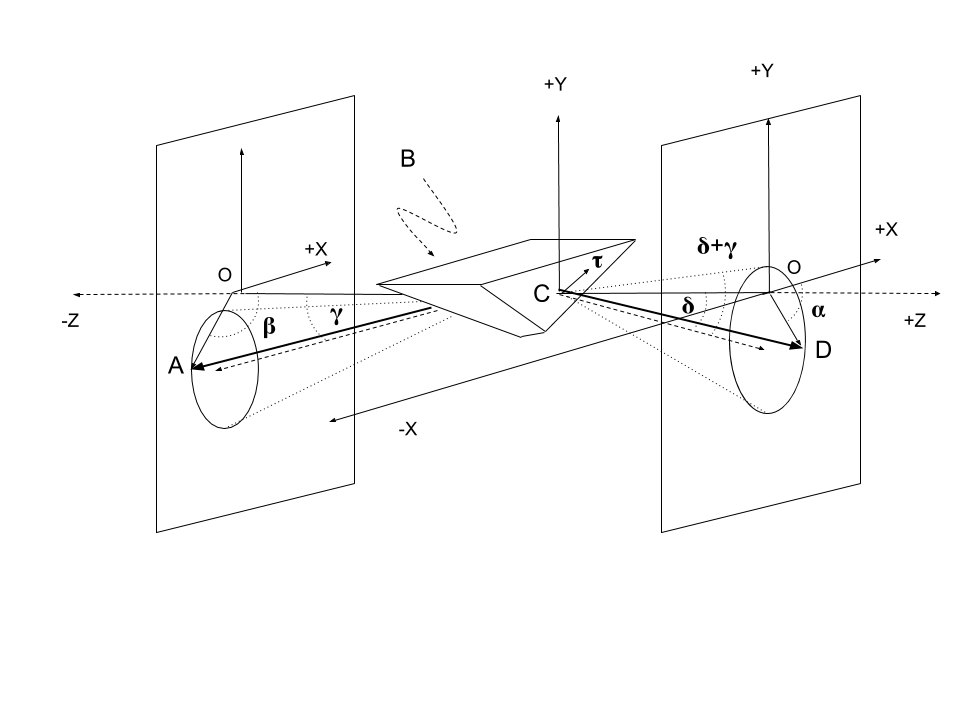
\includegraphics[width=0.80\textwidth]{figures/TwistSpectrumProof.png}
     \caption{Twist Spectrum Proof Diagram}
  \label{fig:twistspectrum}
\end{figure}


\begin{proof}
  Please see Figure \ref{fig:twistspectrum}, which renders and arbitrary
  prism in balanced position. The $B$ joint is on the backside of the
  prism, not visible. As usual, $\tau$ is measured against the
  face. The face normals are labelled $N_b$ and $N_c$. The are drawn
  to projection planes orthogonal to the object axis, which is $z$-axis
  aligned as per our usual convention. The $N_b$ face normal forms
  an angle $\delta$ with negative $z$-axis, and the $N_c$ face normal
  an angle $\gamma$ with the positive $z$-axis.

  Let the function $\alpha(\tau)$ which is the angle formed by the
  projection of $A$ and the orign with the $X$ axis in the $XY$-plane.
  Let $\beta(\tau)$ be the angle of the $D$ projection. $\alpha(\tau)$
  and $\beta(\tau)$ are periodic on $\tau$ ranging between $0$ and
  $2\pi$.

    Let $\gamma$ and $\delta$ be the angle between the $A$ face-vector and
    $B$ face-vectors respectively formed with the
    $\overline{BA}$ vector and $\overline{AB}$ respectively.

    If $\gamma \neq \delta$ then one is greater than the other.
    Without loss of generality, assume $\gamma > \delta$.
    Then $D$ moves in a cone
    about the $N_c$ face normal as $\tau$ is varied. The
    angle of the projection of $D$ is $\beta$, which varies as $\tau$
    varies.
    The projection of both $A$ and $D$ move in circles
    potentially tilted to the $z$-axis, thereby
    forming ellipse-like figures in the projection planes.

    By our assumption, because $\gamma > \delta$, the
    ellipse formed by $D$ as $\tau$ changes
    strictly contains the origin of the projection plane.
    Therefore at least one of $\beta(\tau)$  has a range
    containing both $0$ and $2\pi$, since the angle swept out by
    a point on the edge of this figure goes completely around the origin.
    Without loss of generality, let $\alpha$ have that property.

    Both $\alpha$ and $\beta$ are continuous, by the continuity of
    physcial mechanisms and the composition of continuous functions.

    Note that although the motion need not be proportional, the sign
    of the motion of $\alpha(\tau)$ is the opposite of the sign of the
    motion of $\beta(\tau)$ as $\tau$ is varied.

    Because $\alpha$ varies between $0$ and $2\pi$ (although
    $\beta$ may not), and because $\beta$ moves in the opposite direction,
    by the Intermediate Value Theorem, there is a $\tau$ where
    $\alpha(\tau) = \beta(\tau)$. Such a point produces a toroid-like
    figure.

    Since $\alpha$ can be moved in a complete circle (between 0 and
    $2\pi$), there is always
    exactly one
    $\tau$ which places $\alpha$ oppsite $\beta$
    (i.e., $\alpha = \pi + \beta$). This is the flat case, which
    is the maximal extend of the segmented helix.

    Now let us consider the case that $\gamma = \delta$.
    By our assumption that both there are non-zero $x$ or $y$ components
    to the face normals, $\gamma > 0$ and $\delta > 0$. The figures
    they describe may both contain the origin. However, one of them
    moves through an elliptical figure, and there without loss of
    generality $\beta(\tau)$ sweeps out the full domain between $0$ and
    $2\pi$. By our previous argument, both the torioidal and flat cases
    are found.

    Therefore we can always move continuously through a torus-like
    planar polygon ($\phi = 0$) and a maximally extended flat case.

\end{proof}


It would be more useful and elegant to have a formula for the $\tau$ that produces
a torus as a function of the joint face normals; the authors have not been able
to produce such a formula. However, we in the calculator page, we numerically
provide the $\tau$ that produces the minimum tightness (torus-like) and maximum tightness (zig-zag) to the
nearest degree,
with the labels {\em Minimum Tightness $\tau$} and {\em Maximum Tightness $\tau$}.

\subsection{Qualitative Observations}

When the normals are coplanar vectors, then the minimum tightness $\tau$ is
always $0$, and the maximum tightness occurs when $\tau = \pm \pi$.
These values deviate from $0$ and $\pi$ roughly in proportion
to the non-coplanarity of the normals.

Varying $\tau$ smoothly varies the tightness of the coiling of the helix,
moving through vary linear cases towards a torus,
to a torus, to a very linear case on the other side.

In fact it is possible to that there is always a ``tightest coil''
which does not self-intersect. If we had many objects,
we could pack them into a convenient space by computing the $\tau$
of the tightest coil and stacking them this way.
If we had a means to change $\tau$, perhaps via motors in a robot arm,
we would have a smoothly telescoping and contracting
robot arm or linear actuator.
If we had a repated molecular subunit that changed shape in
response to an exteranl magnetic or electric field or chemicals in the surrounding
environment, we would have a telescoping nanomachine.


\subsection{A Brute-force approach to finding Helix Angle from Twist}

The calculation methods described in this paper hardly warrant the name ``algorithm'' when considered from the computational complexity;
the are all constant time (for a given fixed precision.)
Although involving trigonometric functions, they demand no iteration.

This makes it practical to solve some problems by brute-force iteration.
An example already calculated is the twist $\tau$ which makes
an object product a toroid-like segmented helix, or on the other hand
the $\tau$ value that maximizes linear extent and tightness.
Future work may allow analytic formulae for $\tau$ as a function of
tightness to be developed; but in the meantime it is easy enough
to simply evaluate objects at many different $\tau$ values to find a
desired helix angle $\phi$, such as $0$. One can of course bring
standard numerical optimization to bear, because an objective function
that depends on the parameters of the segmented helix can
be computed in constant time.

\section{Applying to The Boerdijk-Coxeter Tetrahelix}

The Boerdijk-Coxeter tetrahelix is a periodic chain of conjoined regular tetrahedra
which has been much studied\cite{coxeter1985simplicial,sadler2013periodic,fuller1982synergetics,read2018transforming}
and happens to have irrational measures, making it an ideal
test case for our algorithms. Because the face-normals can be calculated and the
positions of the elements of the BC helix directly calculated, we can use
it to test our algorithms, and in fact these algorithms give the same rotation.

However, it should be cautioned that the helix which Coxeter identified\cite{coxeter1985simplicial} goes through every node of every tetrahedron. Constructing the helix that goes
through only ``rail'' nodes allows irregular tetrahelices to be designed\cite{read2018transforming}.
However, the segmented helices defined in this paper do neither; rather, it is most natural to
imagine them moving through the centroid of face of a tetrahedron.
This complementary view is to think of the BC Helix not as the helix that
intersects the vertices of the tetrahedron as Coxeter did\cite{coxeter1985simplicial}, nor a single
rail as may be valuable to engineers\cite{read2018transforming}, but rather as a helix through
the center point of the faces of the tetrahedron. This is a segmented helix of
very small radius ($0.0943$) compared to the other two approaches
($\frac{3\sqrt{3}}{10} \approx 0.5196$) which measure the radius to the
point of the tetrahedron, but it has
the advantage that it is far more general. For example, it is
clearly defined if one used truncated tetrahedra.
The rotation of a
segment matches the BC Helix analytical solution
($\theta = \arctan{-3/2} \approx 131.8103$),
because a screw transformation does not depend on selecting a point for the radius.

In light of Lord's Observation and the Segmented Helix algorithms, we can now
consider the BC Helix and a variety of other segmented helices generated by
face-to-face stacking of Platonic solids, examples of called {\em Platonic segmented helixes},

Note this also makes clear that in these cases we must also specify the {\em twist},
even if we insist on perfect face-to-face matching. Thinking of it this
way, there are actually three tetrahedral segmented helices,
depending on which twist modulo 120$\degree$
is chosen (keeping the faces matching). In the case of the tetrahedron,
this creates the clockwise BC Helix, the anti-clockwise BC Helix, and the
not-quite-closed tetrahedral torus, similar in appearence to but quite the same as
{\em toriodal polyhedra}\cite{wiki:toroidalpolyhedra}.
(Five tetrahedra famously lack $\approx 7.356$ degrees of being a perfect toriodial polyhedron
as can be seen from our sofware which computes $\theta = 70.5288$ for this case,
so the gap is $360 - 5 \cdot \theta \approx 7.356$)

In the case of the icosahedron, there are in fact many possibilities,
as one need not choose the precisely opposite face as the joining face, and
one may choose up to three twists. The ``zoo'' or Platonic helices
can be studied via the calculations described here, and our software
makes these interactively selectable (see Section\ref{sec:platonic}).

\section{Implications}

One of the implications of having an easily-calculable understanding of the math
is that it may be possible to design helices
of any radius and pitch by designing periodic (possibly scalene) segments. Combined with slight
irregularities, this means that you have a basis of design molecular helices
out of ``atoms'' which correspond to our objects.

This would mean that if you wanted to build a brace of length exactly 3 meters
with bars of exactly 1/2 meter you would be able to come as close to this
as mathematically possible.

A modular robot constructed out of repetitions of the same shape-changing module will always product a helix
whose precise shape can be controlled by uniformly changing the shape of all of the modules.

\section{The Platonic Helices}

\label{sec:platonic}

In order to demonstrate the utility of the calculations explained in this paper, we have explored
periodic chains of the five regular Platonic solids joined face-to-face so that their vertices coincide,
which form {\em Platonic helices.}
Such tetrahelices, icosahelices, octahelices and dodechelices
have been mentioned in a number of papers\cite{elgersma2016quadrahelix,babiker2012combinatorial,lord2001sphere}, but not exhaustively studied in
the purely helical form.
We propose the name {\em cubahelix} for the helix made from cubes, as opposed to the equivalent
but cumbersome {\em hexahedronahelix}.
Because in some cases Platonic segmented helices may be found in nature or
related to structures found in nature\cite{lord2004gamma,pearce1990structure},
it would be convenient to have a table, and images, of all such Platonic segmented helices for reference.

To construct a periodic chain from a Platonic solid, one must decide which faces are joined by the rule.
Additionally, one must determine a twist
$\tau$ as part of the rule, and this twist must be chosen from a small set if the vertices are to coincide.
The set of vertex-matching twists differs slightly depending on the face chosen for octahedron, dodacahedron, and icosahedron
(but not for the tetrahedron and the cube.) The number of twists in a set will always be equal to the number of sides on a face.

Therefore the number of Platonic helices is in principle a summation of a number of faces times a number of sides, or
$4 \cdot 3 + 6 \cdot 4 + 8 \cdot 3 + 12 \cdot 5 + 20 \cdot 3 = 12 + 24 + 24 + 60 + 60 = 180$.
However, many of the possibly helices will be indistinguishable of we consider only the shapes produced, as
opposed to considering labeled faces. Furthermore,
every non-toroidal helix will come in clockwise and counter-clockwise version.
However, we do not consider rules such as ``attach face zero to face zero''
which would constitute
``doubling back''\cite{elgersma2016quadrahelix}.
The transformation matrix for such a rule would be the identity matrix.
It produces an object axis of zero length, a radius of zero, and
a travel of zero. It produces perfect self-intersection; that is the entire
degenerate helix would appear to be a simply a single Platonic solid.

Using the math in this paper, it was easy to evaluate all 180 helices,
place them in a table, and group them
by radius and travel (collapsing chirality).
The result is 28 unique shapes. In this number, no provision was made to exclude
self-intersection,
which does occur, but might not matter to
an aerospace engineer building a collapsible space frame of rods and joints.
In the language of Elgersma and Wagon\cite{elgersma2016quadrahelix}, not
all of the 28 Platonic helices {\em embedded}.

With those caveats, the helices in Table \ref{table:platonic}, exemplified by
accompanying figures and renderable
interactively on our calculator page, thus represents an exhaustive catalog,
colloquially called a ``zoo'', of all Platonic helices.

Many of the these helices have been previously individually
mentioned and even rendered in the literature,
though not necessarily fully calculated.
In this table, column {\em C-Face} refers to the
face as numbered by the THREE.js software\cite{dirksen2013learning},
which is somewhat arbitrary. The {\em \# Analogs}
column gives the number of Platonic Helices with the same shape, or the enantiomer of it, that is, the same
shape in either the clockwise or anticlockwise direction. This list can be expanded completely in our interactive software.

Clearly, for each solid there is a change in twist which keeps the faces
aligned if they start aligned. This is the $2\pi/n$,
where $n$ is the number of sides in a face. The base twist that creates
a perfect face-to-face match depends not only on the solid but the face we choose to conjoin to.
For each of the Platonic
solids, we have just computed this base angle by visual inspection and trial and error.
The twist $\tau$ if a species
of helix in given in the column below.

\begin{table}[ht]
\caption{The Platonic Helices} % title of Table
\centering % used for centering table
\begin{tabular}{l l r r r r r r r}
  \hline\hline %inserts double horizontal lines
  Name & Solid & \# Analogs & C-Face \# & $ \tau $ & radius & $ \theta $ & d & $ \phi $ \\ [0.5ex] % inserts table
%heading
  \hline % inserts single horizontal line
Tetrahelix & Tet &	6 &	1 &	-120 &	0.094 &	131.810	& -0.516 & 161.565 \\
Tetratorus & Tet & 	3 &	1 &	0    &	0.471 &	70.529	& 0.000	& 90.000 \\
\hline %inserts single line
Boxbeam & Cub &	4 &	1 &	-180 &	0.000 &	0.000 &	1.000 &	0.000 \\
Staircase & Cub &	4 & 	2 &	-180 &	0.000 &	0.000 &	0.707 &	0.000 \\
Blockhelix & Cub & 	8 & 	2 & 	-90  &	0.236 &	120.000 & -0.577 & 144.736 \\
Cubatorus & Cub &	4 &	2 &	0 &	0.500 &	90.000 & 0.000 & 90.000 \\
\hline %inserts single line
Octabeam & Oct &	3 &	5 &	-60 &	0.000 &	0.000 &	1.155 &	0.000 \\
Octaspikey & Oct &	6 &	1 &	-120 &	0.148 &	146.443 & -0.603 & 154.761 \\
Octamedium & Oct &	6 &	2 &	-120 &	0.163 &	131.810 & -0.894 & 161.565 \\
Octagear & Oct &	3 &	1 &	0 &	0.408 &	109.471 & 0.000	& 90.000 \\
Treestar & Oct &	3 &	2 &	0 &	0.816 &	70.529 & 0.000 & 90.000 \\
\hline %inserts single line
Dodecabeam & Dod &	5 &	8 &	-108 &	0.000 &	0.000 &	1.589 &	0.000 \\
Dodecadoubler & Dod &	10 &	1 &	-144 &	0.113 &	161.301 &-0.805 & 164.550 \\
The Alternater & Dod &	10 &	2 &	-144 &	0.118 &	149.520 &-1.333	& 170.306 \\
Dodecashaft & Dod &	10 &	1 &	-72 &	0.351 &	129.657	&-0.543 & 130.501 \\
Dodecagear & Dod &	5 &	1 &	0 &	0.491 &	116.565	& 0.000	& 90.000 \\
Dodecacorkscrew & Dod &	10 &	2 &	-72 &	0.546 &	93.026 & -1.095 & 144.110 \\
Dodecadonut & Dod &	5 &	2 &	0 &	1.286 &	63.435 & 0.000 & 90.000 \\
\hline %inserts single line
Pearlshaft & Ico &	3 &	13 &	-60 &	0.000 &	0.000 &	1.589 & 0.000 \\
Quasi-planar & Ico &	6 &	8 &	165 &	0.049 &	167.764 & 1.294 & 4.347 \\
Two Strands & Ico &	6 &	1 &	120 &	0.137 &	159.446	& 0.499 & 28.340 \\
Slow Twist & Ico &	6 &	12 &	120 &	0.169 &	124.309	& 1.454	& 11.641 \\
Rock Candy & Ico &	12 &	2 &	120 &	0.204 &	146.443	& 0.830 & 25.239 \\
Icosa Tree Star & Ico &	3 &	1 &	0 &	0.304 &	138.190	& 0.000	& 90.000 \\
Icosacorkscrew & Ico &	6 &	8 &	-75 &	0.512 &	99.253	& -1.037 & 143.042 \\
Planar point cluster & Ico &	6 &	2 &	0 &	0.562 &	109.471 & 0.000 & 90.000 \\
Big Icosacorkscrew  & Ico &	6 &	8 &	45 &	0.803 &	82.064 & 0.756 & 54.343 \\
The Wheel & Ico &	3 &	12 &	0 &	2.080 &	41.810 & 0.000 & 90.000 \\
\hline %inserts single line
\end{tabular}
\label{table:platonic} % is used to refer this table in the text
\end{table}

\subsection{Qualitative Descriptions and Interesting Shapes}

For fun and to facilitate conversation, we have given all
28 of these Platonic helices nicknames that we find descriptive\footnote{These impressions
  are likely to be incomprehensible to a non-native speaker of English, or even to
  somone not born in America in the 1960's. We apologize for this, and hope the value of connoting the shape outweighs this cultural bias.}
A few of these are interesting enough
to be worthy of particular mention, and comparing them
shows the possibility of designing structures using nothing but Platonic solids.
The math in this paper works equally well with irregular shapes as well,
allowing continuous spectra of designed structures from repeated shapes
or molecules.

\begin{itemize}
\item ``The Blockhelix'' (Figure \ref{fig:blockhelix}) is cubic rectilinear structure in which all angles are right angles; nonetheless
  a segmented helix hides inside it perhaps not apparent to the human eye at first glance.
\begin{figure}
     \centering
     \includegraphics[width=0.40\textwidth]{figures/Blockhelix.png}
     \caption{The Blockhelix}
  \label{fig:blockhelix}
\end{figure}

\item ``Pearlshaft'' (Figure \ref{fig:pearlshaft}). Conjoining parallel faces always produces a {\em shaft}. This icosahedron, being relatively round,
  resembles a string of pearls.
\begin{figure}
     \centering
     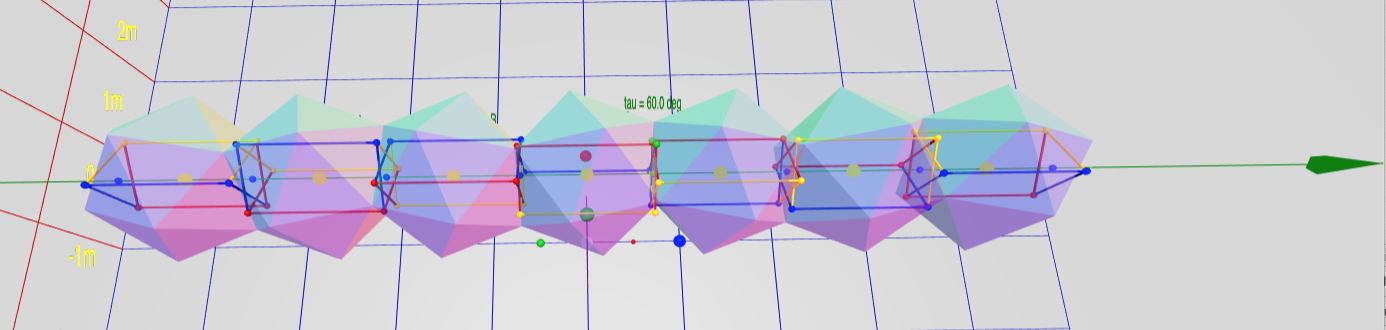
\includegraphics[width=0.40\textwidth]{figures/PearlShaft.png}
     \caption{The Pearlshaft}
  \label{fig:pearlshaft}
\end{figure}

\item However, shaft-like helices exist which do not join opposite faces. ``The Dodecashaft'' (Figure \ref{fig:dodecashaft}) is a remarkably tight
  non-self-intersecting dodecahelix with very narrow gaps between objects.
  Such a configuration
  might be formed by nanofibers under pressure.
\begin{figure}
     \centering
     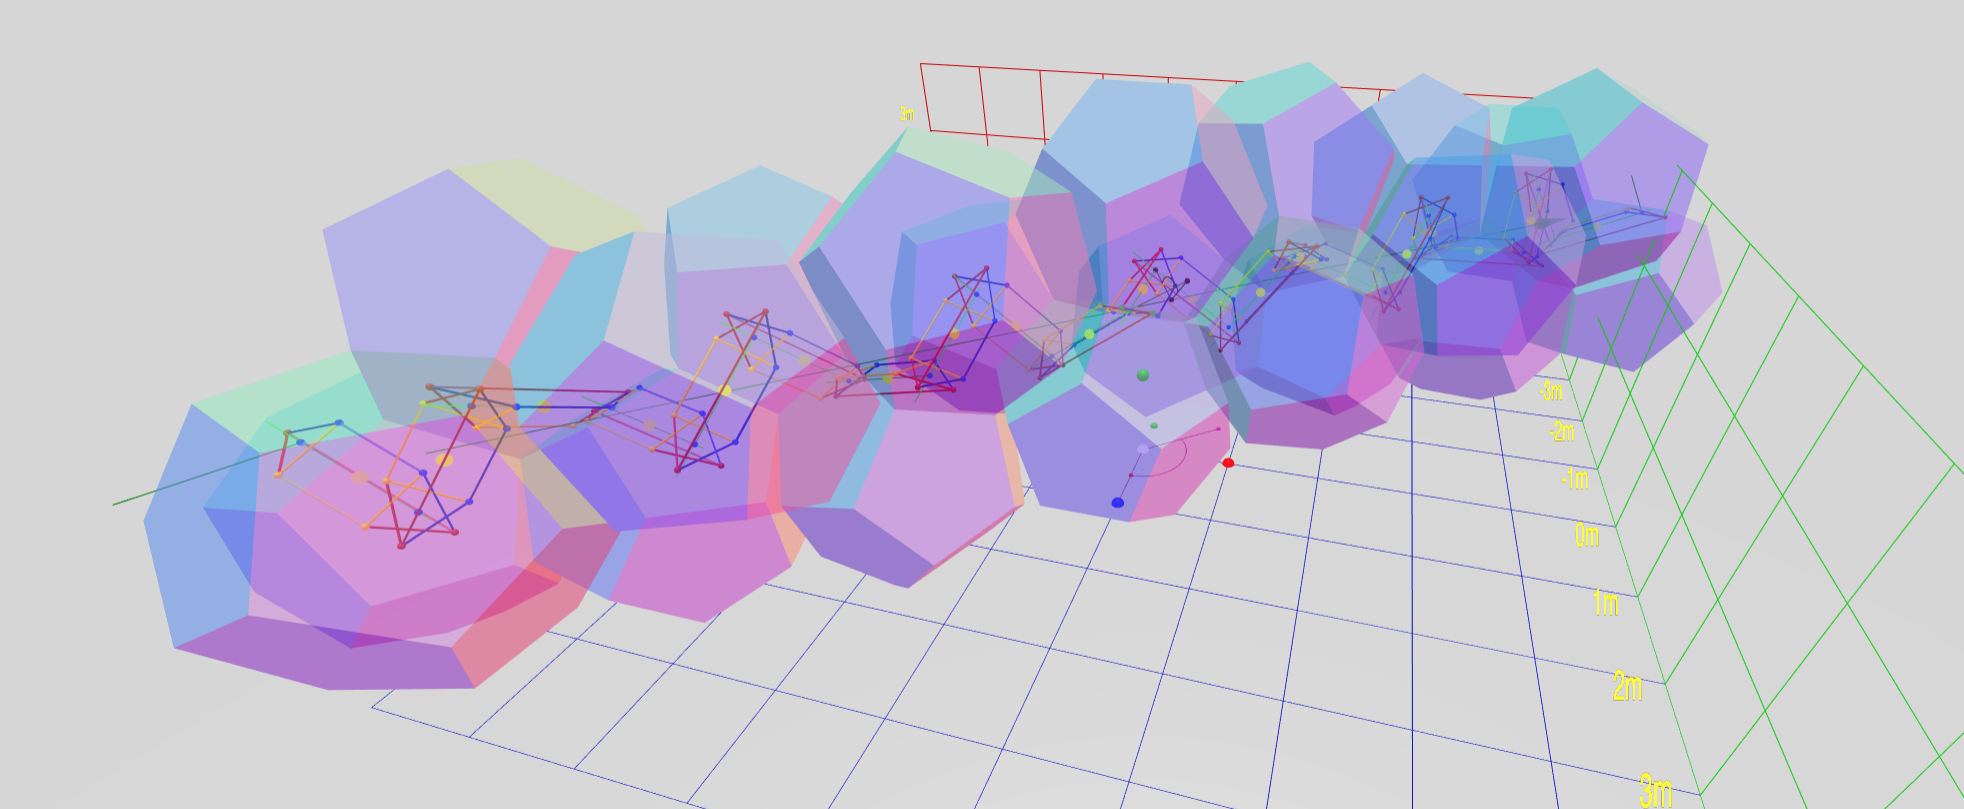
\includegraphics[width=0.40\textwidth]{figures/Dodecashaft.png}
     \caption{The Dodecashaft}
1  \label{fig:dodecashaft}
\end{figure}
\item ``The Dodecadoubler'' (Figure \ref{fig:dodecadoubler}) presents the appearance of being a double helix, even though in fact it is a single helix with
  a simple twist of 72 $\degree$ from the Dodecashaft
\begin{figure}
     \centering
     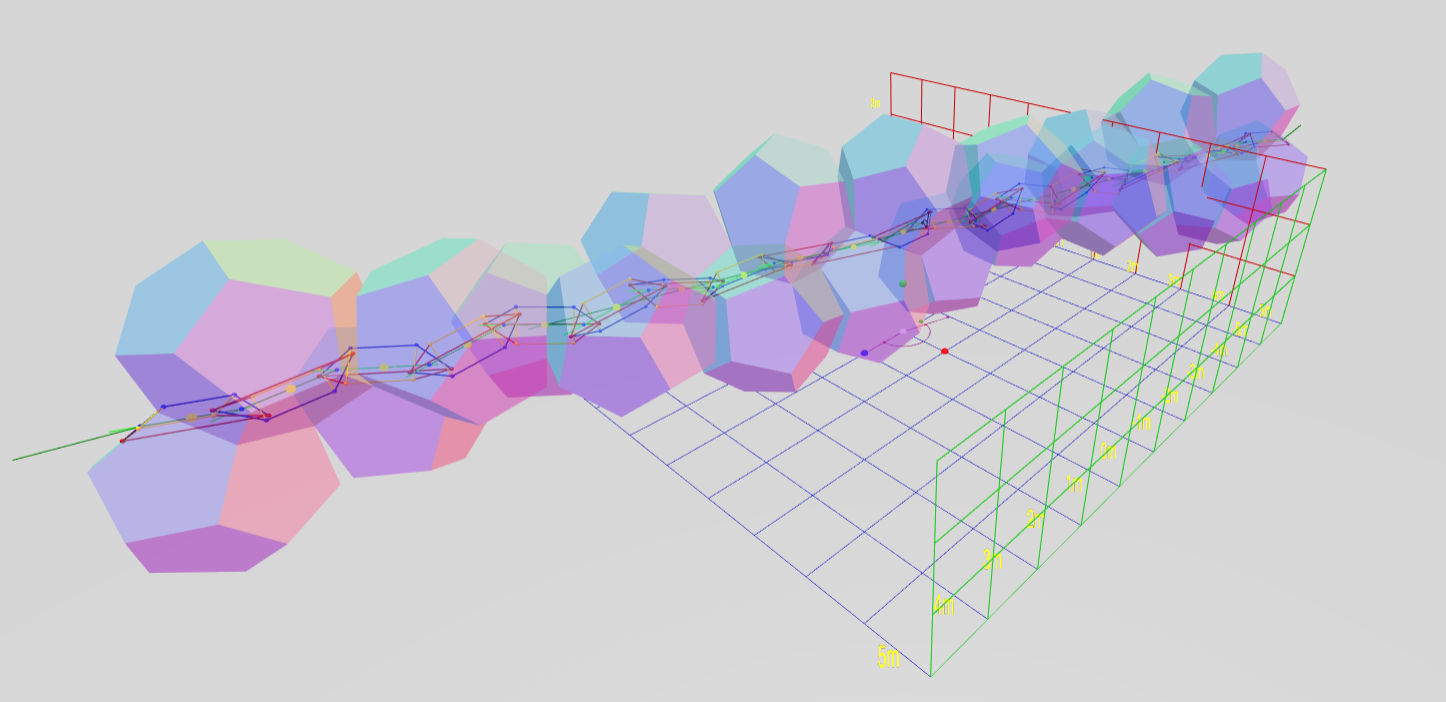
\includegraphics[width=0.40\textwidth]{figures/Dodecadoubler.png}
     \caption{The Dodecadoubler}
  \label{fig:dodecadoubler}
\end{figure}
\item ``The Dodecacorkscrew'' (Figure \ref{fig:dodecacorkscrew}) is a contrasting example of a loose helix, reminiscent of a corkscrew for opening wine bottles.
\begin{figure}
     \centering
     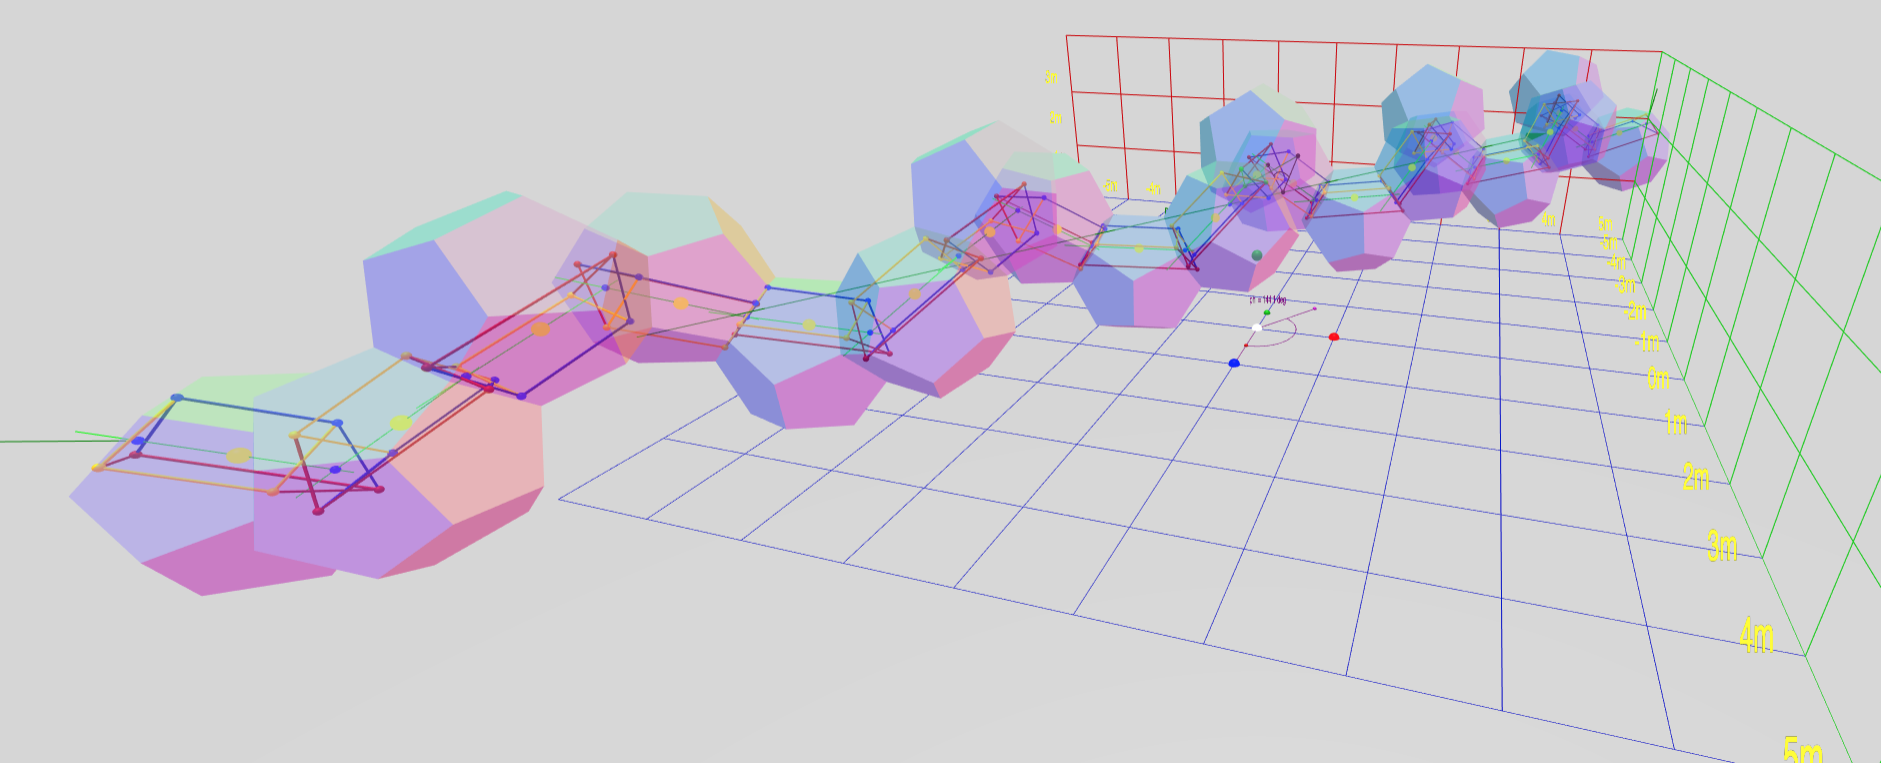
\includegraphics[width=0.40\textwidth]{figures/Dodecacorkscrew.png}
     \caption{The Dodecacorkscrew}
  \label{fig:dodecacorkscrew}
\end{figure}
\item The ``Quasi-planar'' (Figure \ref{fig:quasiplanar}) icoshelix presents a slowly twisting metahelix, so perhaps 10 icosahedron could be said to ``lay flat''. If this were
  a molecule or a physical structure made of less-than-perfect rigid members it migt be possible to force it into a pure planar configuration,
  thus wrapping a cylinder or a plane, studding it with icosahedra.
\begin{figure}
     \centering
     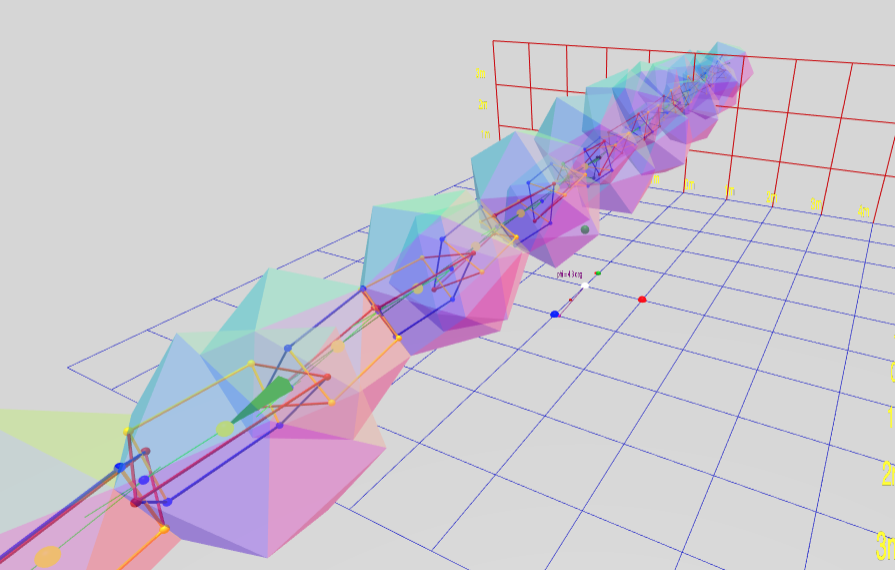
\includegraphics[width=0.40\textwidth]{figures/Planar.png}
     \caption{Quasi-planar icosahelix}
  \label{fig:quasiplanar}
\end{figure}
\item ``Two Strands'' (Figure \ref{fig:twostrands})is similar to the ``Dodecadoubler'' but even more
  visually striking. It is reminiscent of a depictions of a DNA double
  helix.
\begin{figure}
     \centering
     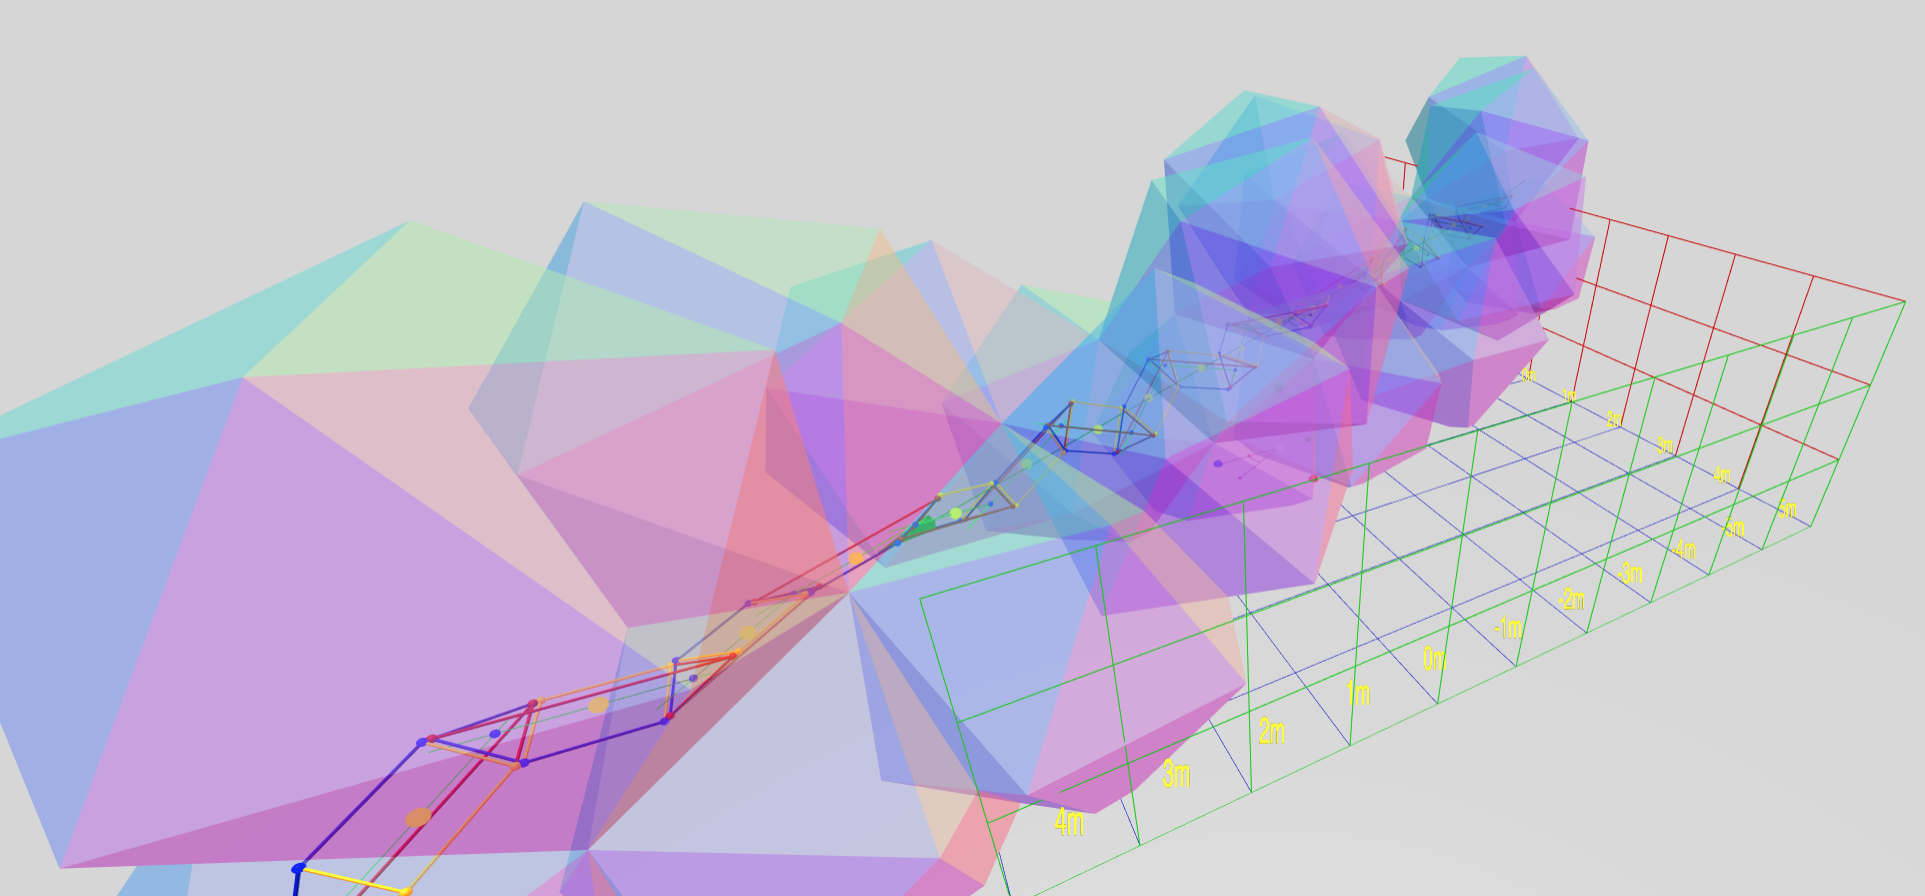
\includegraphics[width=0.40\textwidth]{figures/TwoStrands.png}
     \caption{Two Strands}
  \label{fig:twostrands}
\end{figure}
\item ``The Wheel'' (Figure \ref{fig:thewheel}) resembles a modern car tire
  in proportions.
  All Platonic solids and indeed all shapes have torus-like
  configurations. In general they do not ``close'' perfectly; that is, there is a gap that prevents the final faces from fitting together perfectly.
  However, one could make tiny adjustment to repeated shape to close this gap.
\begin{figure}
     \centering
     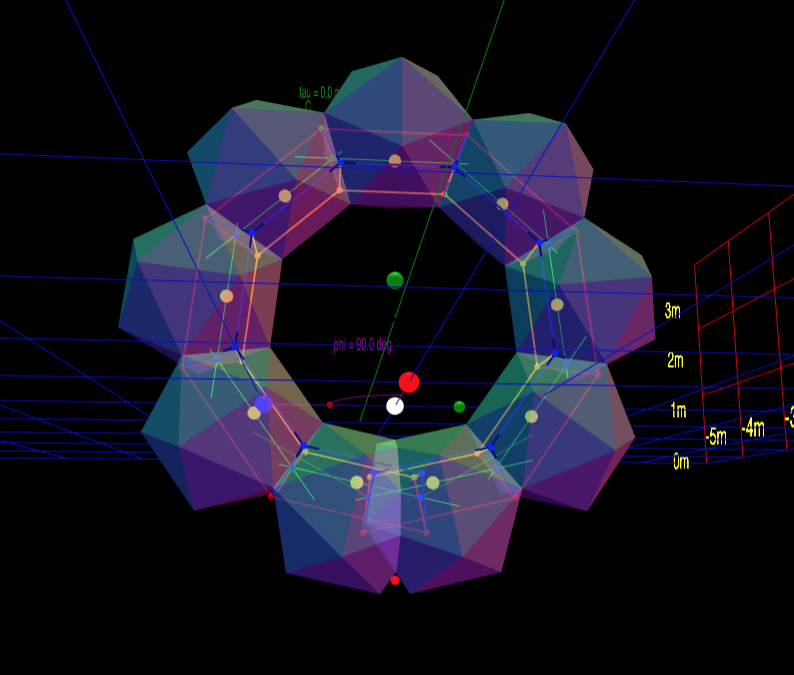
\includegraphics[width=0.40\textwidth]{figures/TheWheel.png}
     \caption{The Wheel}
  \label{fig:thewheel}
\end{figure}
\end{itemize}

\section{Future Work}

The algorithms and software described herein allow numerical calculation of the intrinsic properties of these
Platonic helices, but it would be even better to describe them in with closed-form expressions,
as Coxeter did for the Boerdijk-Coxeter tetrahelix.
The math and the algorithms are simple enough that if coded in a symbolic algebra system like Mathematica,
or with careful work, closed-form
expressions could be produced for all the regular Platonic helices.
These would be interesting if they happen to be short; we have no reason to
believe they will be. The same work could be done for the Archimedean solids. The current work would
serve as a useful validation check and intuition-builder for such work.

There may exist a closed-form expression for twist $\tau$ which produces a desired helix angle $\psi$; we have provided only
an iterative algorithm for it, which is practical but less elegant.

\section{ To Do}

\begin{itemize}
  \item MAJOR BUG: C.z < 0 and B.z < 0 causes mismatch
\item Consider application here: https://imbicorg.blogspot.com/p/the-main-objective-of-conference-is-to.html
  \item Here: http://www.ramsaconference.com/
\item Add sidedness to our calculations?
  \item
  \item Modify that so that it truly respects $\psi$ as an input.
\item Provide explanation, graphically, if need be, for
  the computation of $B_{ax}, B_{ay}, B_{az}$ in the general cases.
\item Clean up the code. 3 days
\item Go through each reference 1 day
\item Try to get list of references to the computation of a screw from an arbitrary matrix, and compare and contrast to our code. 1 day
\item Need to understand possibility of further simplifying specification of object.

\item Need to get this paper, by hook or by crook, and probably cite:
  Note: An historical review of the theoretical development of rigid body displacements from Rodrigues parameters to the finite twist
  \url{https://www.sciencedirect.com/science/article/pii/S0094114X0500087X}
  \item Improve qualitative section, talk about toruses - 8 hours
  \item Consider better naming mechanism for faces - 4 hours
  \end{itemize}

\section{References that need to be studied or reviewed}


Note further that Equations 7 and 8 of this paper\cite{kahn1989defining} give BETTER equations for radius $r$ and the distance $d$ than what I have so far given. Note: I've studied this; I'm not sure there is anything worth doing there.

This is a discussion of segmented coils in a protein structure:

\url{https://www.sciencedirect.com/science/article/pii/0022283688903701}

A modern helix structure protein paper:

\url{https://www.sciencedirect.com/science/article/pii/S1476927108000583}


``Simulation of Suspensions of Helical Rigid Fibers'' Y Al-Hassan : British Journal of Mathematics and Computer Science
(PDF downloaded)

``HELFIT: Helix fitting by a total least squares method'' : This needs to be studied closely!
\url{https://www.sciencedirect.com/science/article/pii/S1476927108000418}

QHELIX: A Computational Tool for the Improved Measurement of Inter-Helical Angles in Proteins
\url{https://link.springer.com/article/10.1007/s10930-007-9097-9}

Note:''On the Screw Axes and Other Special Lines Associated With Spatial Displacements of a Rigid Body''
\url{http://manufacturingscience.asmedigitalcollection.asme.org/article.aspx?articleid=1439697}

Note: An historical review of the theoretical development of rigid body displacements from Rodrigues parameters to the finite twist
\url{https://www.sciencedirect.com/science/article/pii/S0094114X0500087X}


\section{Acknowledgements}

Thanks to Prof. Eric Lord for his direct communication.

The enthusiasm of the participants of the 2018 Public Invention Mathathon
intitiated this work.

\bibliographystyle{unsrt}
\bibliography{shelix}

\appendix


\end{document}

\section{References Reviewed but not worth citing}

This is a long, expensive book, but it is not relevant relevant\cite{hyde1996language}:
\url{https://books.google.com/books?hl=en&lr=&id=1LZlSZ7ORrQC&oi=fnd&pg=PP1&ots=0hSEwJvlUB&sig=xNG9UWv_H1OXHwaOiOBJN7TW6xA#v=onepage&q&f=false}


Note: There is another long, deep book that needs to be obtained and studied\cite{sadoc2006geometrical}.
\url{https://books.google.com/books?hl=en&lr=&id=FHPlDWvz1bEC&oi=fnd&pg=PP1&ots=TsOnodavEZ&sig=HO86UUVlqRVWGqY-Tv02nb7x7NA#v=onepage&q&f=false}


This talks about tuning the period of a helix inside a nanopore:

\url{https://aip.scitation.org/doi/abs/10.1063/1.4794785}



\url{https://www.researchgate.net/publication/236066626_Segmented_helical_structures_formed_by_ABC_star_copolymers_in_nanopores}


``Local Frustration Determines Molecular and Macroscopic Helix Structures''

\url{https://pubs.acs.org/doi/abs/10.1021/jp4040503}


NOTE: This is a discussion of representing joint angles, it is not obvious how valuable it is:
\url{https://www.clinbiomech.com/article/S0268-0033(98)00080-1/abstract}

\url{https://www.win.tue.nl/~wstomv/publications/mathmitering-final.pdf}


\url{https://gist.github.com/peteristhegreat/3b76d5169d7b9fc1e333}

\url{https://www.sciencedirect.com/science/article/pii/S0022309307005583}


This reference is EXTREMELY IMPORTANT
\url{https://link.springer.com/article/10.1023/A:1015863923728}



This may be worth reading:
\url{https://link.springer.com/article/10.1007/PL00011063}

Some discussion of ``screw transformations''
\url{http://dergipark.gov.tr/download/article-file/56483}

``Analyzing Protein Structure Using Almost Delaunay Tetrahedra''

\url{https://www.researchgate.net/profile/Alexander_Tropsha/publication/250901525_Analyzing_Protein_Structure_Using_Almost-Delaunay_Tetrahedra/links/5578584408ae75215870347c/Analyzing-Protein-Structure-Using-Almost-Delaunay-Tetrahedra.pdf}
